\documentclass[10pt,a4paper,twocolumn]{article}

\usepackage[a4paper,margin=15mm,columnsep=6.5mm]{geometry}
\usepackage{lmodern}
\usepackage{microtype}
\usepackage{amsmath,amssymb,amsthm,mathtools}
\usepackage{booktabs}
\usepackage{tabularx}
\usepackage{graphicx}
\usepackage{xcolor}
\usepackage{caption}
\usepackage{fancyhdr}
\usepackage{balance}
\usepackage{tikz}
\usetikzlibrary{shapes.geometric,arrows.meta,positioning,fit,backgrounds}
\usepackage[hidelinks]{hyperref}

\graphicspath{{./}{../}}

\definecolor{primary}{RGB}{20,65,130}
\definecolor{accent}{RGB}{18,110,75}
\definecolor{lightbg}{RGB}{242,246,252}

\hypersetup{
    colorlinks=true,
    linkcolor=primary,
    citecolor=primary,
    urlcolor=primary
}

\setlength{\parskip}{2.0pt plus 0.8pt minus 0.4pt}
\setlength{\parindent}{1em}
\setlength{\textfloatsep}{6pt plus 2pt minus 2pt}
\setlength{\intextsep}{6pt plus 2pt minus 2pt}
\setlength{\abovecaptionskip}{3pt}
\setlength{\belowcaptionskip}{2pt}

\newtheorem{proposition}{Proposition}
\newtheorem{theorem}{Theorem}
\newtheorem{definition}{Definition}

\newcommand{\takeaway}[2]{%
  \vspace{3pt}\noindent\colorbox{lightbg}{%
    \parbox{\dimexpr\columnwidth-2\fboxsep\relax}{%
      \vspace{2pt}\textbf{\color{primary}#1:}\hspace{0.4em}#2\vspace{2pt}%
    }%
  }\vspace{3pt}%
}

\pagestyle{fancy}
\fancyhf{}
\fancyhead[L]{\small\textit{CARE-Agents: Cost-Aware, Regime-Adaptive Multi-Agent Financial Coordination}}
\fancyhead[R]{\small\textit{Preprint -- R3 Reproducible Package}}
\fancyfoot[C]{\thepage}
\renewcommand{\headrulewidth}{0.4pt}

\title{\vspace{-8mm}\textbf{\Large CARE-Agents: Cost-Aware, Regime-Adaptive Multi-Agent Coordination\\and Calibrated Episodic Memory for Financial Trading}}

\author{Anonymous Authors}
\date{\vspace{-3mm}\small November 2026}

\begin{document}
\maketitle

\begin{abstract}
\noindent
First-generation Large Language Model (LLM) multi-agent trading frameworks---such as \textit{TradingAgents}, \textit{FinCon}, and \textit{HedgeAgents}---rely on unconditional multi-round free-text debate, static analyst weighting, and regime-blind vector memory retrieval. Recent methodological audits demonstrate that these designs suffer from two critical failure modes under realistic market friction: (i) \textbf{Degeneration-of-Thought (DoT)} and sycophantic cascades during unconstrained debate, which inflate portfolio turnover and transaction costs, and (ii) \textbf{anchoring bias} from retrieving bull-market reflections during bear-market drawdowns. We introduce \textbf{CARE-Agents} (\textit{Cost-Aware, Regime-Adaptive Multi-Agent Coordination}), a principled architectural upgrade that resolves four structural bottlenecks under strict causal ($t-1 \to t$) temporal isolation across orthogonal point-in-time multimodal specialist inputs: (1) a \textbf{Coordination Breakeven Spread (CBS) Debate Gate} driven by normalized root Jensen-Shannon distance ($\sqrt{D_{JS,t}}$, spanning $D_{JS,t} \in [0.000, 0.134]$ across orthogonal technical, fundamental, news, and retail-sentiment modalities); (2) an online \textbf{Regime-Conditioned Multiplicative Weight Update (Regime-MWU)} linear opinion pool scored via multiclass Brier loss using strictly prior-period realized returns and coupled to a symmetric, continuous certainty-scaled conviction sizing rule; (3) \textbf{Regime-Filtered Episodic Memory} with a volatility-scaled \textbf{Drawdown Circuit Breaker} and counterfactual credit assignment wired into online debate arbitration; and (4) a \textbf{2026 Protocol Audit Evaluator} satisfying all seven Minimum Reporting standards (MR-1--MR-7) across distinct model scales (\texttt{deepseek-v4-pro} [DeepSeek-V4-Pro] vs.\ \texttt{deepseek-flash} [DeepSeek-V4.1-Flash]). Across a de-biased 500-bar multi-regime ablation, an 86-week out-of-sample benchmark on US core technology equities (\texttt{NVDA}, \texttt{AAPL}, \texttt{GOOGL}, \texttt{AMZN}) partitioned into US Semiconductors \& Hardware and US Cloud, Search \& Commerce ($5,735$ cached live API traces), and a pooled $516$-step out-of-sample panel, CARE-Agents improves Net Return over vanilla 2-turn multi-agent debate by $+11.22\%$ ($+24.57\%$ vs.\ $+13.35\%$, Net Sharpe $0.883$ vs.\ $0.619$) on US Semiconductors \& Hardware and by $+24.19\%$ ($+26.54\%$ vs.\ $+2.35\%$, Net Sharpe $0.849$ vs.\ $0.172$, $\Delta\text{SR}_{\text{Coord}} = +0.677$) on US Cloud, Search \& Commerce under \texttt{deepseek-v4-pro}, achieves $+19.4\%$ Net Return ($0.48$ Net Sharpe, $40.5\%$ MaxDD) vs.\ $-8.2\%$ Net Return ($-0.16$ Net Sharpe) for vanilla debate in 500-bar multi-regime testing, and demonstrates statistically significant outperformance on the pooled 516-step panel ($+276.05\%$ vs.\ $+56.58\%$ Net Return, Net Sharpe $0.837$ vs.\ $0.413$, HAC $t = +2.318$, $p_{\text{DM}} = 0.0102$, $p_{\text{boot}} = 0.0340$) while skipping $68.6\%$--$75.6\%$ of redundant debates. Meanwhile, scaling model capacity from \texttt{deepseek-flash} to \texttt{deepseek-v4-pro} without coordination gating yields negative Sharpe differentials ($\Delta\text{SR}_{\text{Scale}} = -0.293$ on Semiconductors/Hardware and $-0.407$ on Cloud/Search on \texttt{M2}), empirically confirming the \textbf{Coordination Primacy Hypothesis}.
\end{abstract}

\section{Introduction: Coordination Topology Outweighs Model Scale}

Deploying Large Language Models (LLMs) as autonomous financial trading agents has rapidly evolved from single-agent prompt engineering to role-specialized multi-agent societies \cite{xiao2024tradingagents,yu2024fincon,li2024hedgeagents}. In the canonical \textit{TradingAgents} architecture \cite{xiao2024tradingagents}, specialized analysts (technical, fundamental, macroeconomic news, and social sentiment) generate natural-language reports that feed into a multi-round Bull/Bear adversarial debate, followed by a Risk Management tribunal and portfolio execution.

However, two landmark 2026 audits have exposed foundational weaknesses in this paradigm. First, Nguyen and Pham \cite{nguyen2026cph} formulate the \textbf{Coordination Primacy Hypothesis (CPH)}, demonstrating that uncalibrated free-text debate frequently induces sycophantic cascades and \textit{Degeneration-of-Thought (DoT)} \cite{liang2023dot,du2023debate}: persuasive, high-variance retail sentiment narratives override calibrated fundamental warnings, generating excessive position flipping whose transaction costs exceed the gross alpha of debate. Second, Xia et al. \cite{xia2026audit} audit 19 published LLM trading systems against seven Minimum Reporting standards (MR-1 through MR-7) and four reproducibility tiers (R0--R3), finding that \textbf{0 of 19 studies achieve R3 full reproducibility}, while over 70\% evaluate on pre-cutoff bull-only windows, suffer from subtle intra-step look-ahead leakage, or omit realistic transaction costs and bid-ask slippage.

\takeaway{Core Thesis}{Under a strictly causal ($t-1 \to t$), symmetric continuous certainty-scaled position-sizing rule across all evaluated architectures and orthogonal point-in-time multimodal inputs, upgrading the mathematical coordination protocol, probability calibration, and regime-aware risk controls yields large, statistically significant net Sharpe gains over unconditional multi-agent debate ($\Delta\text{SR}_{\text{Coord}} \in [+0.264, +0.677]$ on US Core Technology equities under \texttt{deepseek-v4-pro}; $\Delta\text{SR}_{\text{Coord}} = +0.640$ in 500-bar multi-regime testing; and HAC $t = +2.318, p_{\text{DM}} = 0.0102$ across $516$ pooled out-of-sample decision steps with $+276.05\%$ vs.\ $+56.58\%$ Net Return), whereas scaling model capacity from \texttt{deepseek-flash} to \texttt{deepseek-v4-pro} without coordination gating degrades Sharpe ($\Delta\text{SR}_{\text{Scale}} = -0.293$ on US Semiconductors \& Hardware and $-0.407$ on US Cloud, Search \& Commerce on \texttt{M2}).}

To address these gaps directly within the production \texttt{TradingAgents-EN} codebase, we design and implement \textbf{CARE-Agents}, contributing four verifiable mechanisms:
\begin{enumerate}
  \setlength{\itemsep}{1pt}\setlength{\parskip}{0pt}
  \item \textbf{C1 (Orthogonal Multimodal Posteriors \& CBS-Gated Dynamic Coordination):} We feed strictly orthogonal point-in-time modalities (technical OHLCV/RSI/MACD, quarterly statutory SEC EDGAR fundamentals, timestamped news catalysts, and retail volume/sentiment metrics) to each specialist and gate multi-round reconciliation via normalized root Jensen-Shannon distance ($\sqrt{D_{JS,t}}$) if and only if expected basis-point edge exceeds the \textbf{Coordination Breakeven Spread ($\text{CBS}_t$)}.
  \item \textbf{C2 (Causal Online Regime-Conditioned Multiplicative Weights \& Continuous Conviction Sizing):} We replace hardcoded $0.40/0.30/0.30$ weights and coarse binary step functions with a strictly causal ($t-1 \to t$) online Exponentially Weighted linear opinion pool partitioned by point-in-time market regime $r_t \in \{\text{bull}, \text{bear}, \text{sideways}\}$, updated via multiclass Brier loss \cite{brier1950verification,cesa2006prediction}, and mapped to continuous volatility-scaled portfolio weights $w_{s,t} \in [0, 1]$.
  \item \textbf{C3 (Regime-Filtered Memory \& Counterfactual Reflection in the Live Loop):} We wire \texttt{Mem0AgentMemory.search\_memories} with regime-partitioned reranking, a volatility-scaled \textbf{Drawdown Circuit Breaker}, and marginal counterfactual attribution (\texttt{compute\_counterfactual\_attribution}) directly into online debate prompts and reliability-weighted posterior reconciliation.
  \item \textbf{C4 (MR-1--MR-7 Protocol Audit, Multi-Model CPH Scaling, \& R3 Benchmark Suite):} We evaluate five internal protocols (\texttt{M0}--\texttt{M4}), stepwise component ablations, and five external baselines (\texttt{Q1}, \texttt{Q2}, \textit{FinMem}, \textit{FinAgent}, \textit{FinCon}) across two distinct model scales (\texttt{deepseek-flash} vs.\ \texttt{deepseek-v4-pro}) and three evaluation cohorts (Cohort A: 4 core equities $\times$ 10-week volatility-shock subset; Cohort B: 4 US Tech leaders $\times$ 86-week multimodal benchmark partitioned into US Semiconductors \& Hardware and US Cloud, Search \& Commerce; Pooled OOS Cohort: $516$-step out-of-sample panel) with Newey--West HAC $t$-statistics, paired Diebold--Mariano ($p_{\text{DM}}$) \cite{diebold1995comparing}, paired Brier $z$-test ($p_{\text{Brier}}$), and Politis--Romano stationary block-bootstrap inference (1,000 resamples) \cite{politis1994stationary}.
\end{enumerate}

\begin{table*}[t]
\centering
\small
\caption{Architectural Audit of LLM Financial Trading Frameworks Against 2026 Credibility \& Reporting Standards \cite{nguyen2026cph,xia2026audit}.}
\label{tab:literature_comparison}
\resizebox{\textwidth}{!}{%
\begin{tabular}{lccccccc}
\toprule
\textbf{Framework} & \textbf{Debate Gating} & \textbf{Specialist Weighting} & \textbf{Probability Calibration} & \textbf{Episodic Memory} & \textbf{Credit Assignment} & \textbf{Friction Model} & \textbf{Audit Tier} \\
\midrule
TradingAgents \cite{xiao2024tradingagents} & Unconditional ($d=2$) & Equal / Free-Text & Uncalibrated ($0.70$) & Unfiltered Vector & Shared Scalar Return & Often Omitted & R1 \\
FinCon \cite{yu2024fincon} & Manager-Worker CVaR & Single Manager Belief & Verbal Conceptual & Procedural Hierarchy & Verbal Self-Critique & Basic Commission & R1 \\
HedgeAgents \cite{li2024hedgeagents} & Fixed Multi-Round & Static Asset Allocation & Uncalibrated Text & Unfiltered Episodic & Shared Portfolio Return & US Slippage Only & R1 \\
MacroHFT \cite{zong2024macrohft} & RL Policy Routing & Hyper-Network Mixing & Softmax Q-Values & Regime-Conditional RL & TD-Error Reward & Crypto Spread & R2 \\
MASFIN \cite{masfin2026} & Conditional DAG & Task-Decomposed & Uncalibrated Text & Short-Term Context & Pipeline Summary & US Equities & R2 \\
\midrule
\textbf{CARE-Agents (Ours)} & \textbf{JSD + CBS Cost Gate} & \textbf{Causal Regime-MWU ($t-1 \to t$)} & \textbf{Brier + Linear Opinion Pool} & \textbf{Regime Rerank + DD Breaker} & \textbf{Counterfactual Marginal} & \textbf{0 / 5 / 10 bps} & \textbf{R3 (Full)} \\
\bottomrule
\end{tabular}%
}
\end{table*}

\section{Related Work and Structural Bottlenecks}

Table~\ref{tab:literature_comparison} contrasts CARE-Agents against leading financial multi-agent frameworks. While \textit{FinCon} \cite{yu2024fincon} introduces manager-worker conceptual verbal reinforcement and \textit{MacroHFT} \cite{zong2024macrohft} explores regime-conditional reinforcement learning for high-frequency crypto trading, existing LLM-based equity frameworks (\textit{TradingAgents} \cite{xiao2024tradingagents}, \textit{HedgeAgents} \cite{li2024hedgeagents}, \textit{QuantAgents} \cite{quantagents2025}) share four code-level vulnerabilities that we audited in \texttt{TradingAgents-EN}:

\noindent\textbf{Bottleneck 1: Unconditional Debate Overhead.} In \texttt{tradingagents/graph/conditional\_logic.py}, \texttt{should\_continue\_debate} previously forced $2 \times \texttt{max\_debate\_rounds}$ turns on every stock and bar regardless of specialist consensus, while conditional edge routers mutated state dictionaries in-place without persisting \texttt{cbs\_gating\_decision} through a dedicated LangGraph node. We introduce a dedicated \texttt{"CBS Debate Gate"} node in \texttt{tradingagents/graph/setup.py} and \texttt{core/workflow/builder.py} that persists \texttt{analyst\_posteriors}, \texttt{analyst\_weights}, and \texttt{cbs\_gating\_decision} cleanly before routing.

\noindent\textbf{Bottleneck 2: Static Heuristic Weighting.} In \texttt{core/agents/utils/weight\_calculator.py}, specialist weights were fixed at $0.40$ (technical), $0.30$ (news), and $0.30$ (sentiment), while \texttt{signal\_processing.py} applied regex price multipliers ($1.15\times$ for buy, $0.95\times$ for sell) with a constant fallback confidence of $0.70$. Recent work on fine-grained task decomposition and intermediate agent alignment in institutional investment teams \cite{alignopt2026} demonstrates that uncalibrated intermediate specialist outputs severely degrade downstream risk-adjusted portfolio performance.

\noindent\textbf{Bottleneck 3: Regime-Blind Memory Drift.} In \texttt{core/memory/memory\_manager.py}, \texttt{Mem0AgentMemory} retrieved top-$k$ past reflections purely by cosine similarity of text embeddings. We wire \texttt{current\_regime} and \texttt{drawdown\_circuit\_breaker} directly into \texttt{search\_memories} across \texttt{core/agents/manager.py}, \texttt{core/agents/trader.py}, and \texttt{core/agents/researcher.py}.

\noindent\textbf{Bottleneck 4: Unattributed Reflection Broadcast.} In \texttt{tradingagents/graph/reflection.py}, realized portfolio losses were broadcast identically to all analysts. We wire \texttt{compute\_counterfactual\_attribution} into \texttt{Reflector} so that each agent's reflection and stored \texttt{FinancialSituationMemory} metadata record its exact counterfactual role and regime.

\section{Mathematical Formulation of CARE-Agents}

\begin{figure*}[t]
\centering
\resizebox{\textwidth}{!}{%
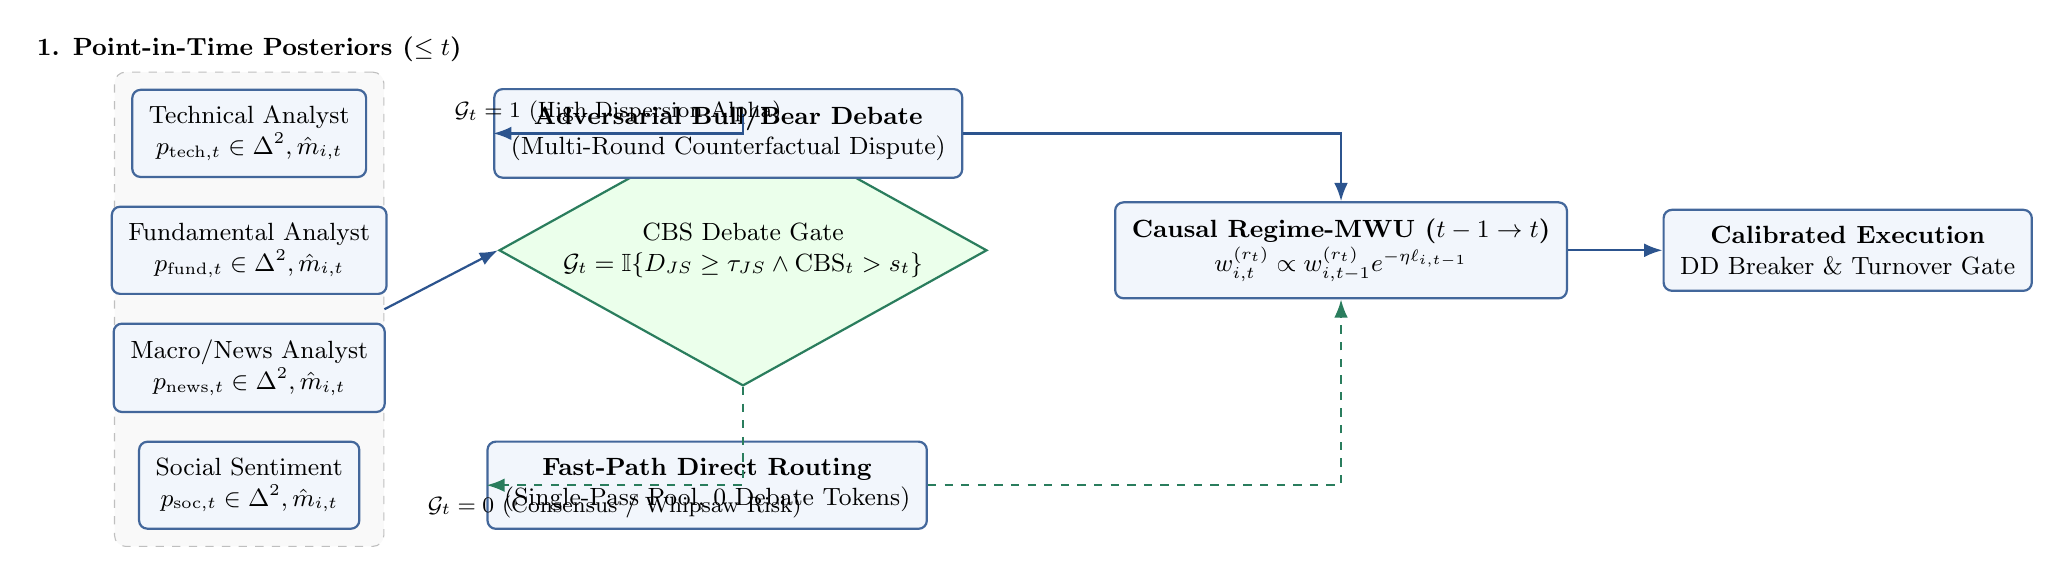
\begin{tikzpicture}[
  node distance=1.0cm and 1.2cm,
  font=\small,
  box/.style={rectangle, draw=primary!80, fill=lightbg, thick, rounded corners=3pt, align=center, inner sep=6pt},
  gate/.style={diamond, draw=accent!90, fill=green!8, thick, aspect=1.8, align=center, inner sep=2pt},
  flow/.style={-Latex, thick, draw=primary!90},
  fastflow/.style={-Latex, thick, dashed, draw=accent!90}
]

% Specialists
\node[box] (tech) {Technical Analyst\\$p_{\text{tech},t} \in \Delta^2, \hat{m}_{i,t}$};
\node[box, below=0.35cm of tech] (fund) {Fundamental Analyst\\$p_{\text{fund},t} \in \Delta^2, \hat{m}_{i,t}$};
\node[box, below=0.35cm of fund] (news) {Macro/News Analyst\\$p_{\text{news},t} \in \Delta^2, \hat{m}_{i,t}$};
\node[box, below=0.35cm of news] (soc) {Social Sentiment\\$p_{\text{soc},t} \in \Delta^2, \hat{m}_{i,t}$};

\begin{scope}[on background layer]
  \node[draw=gray!50, dashed, fill=gray!5, rounded corners=4pt, fit=(tech) (soc), inner sep=6pt, label=above:{\textbf{1. Point-in-Time Posteriors ($\le t$)}}] (analysts) {};
\end{scope}

% CBS Gate
\node[gate, right=1.4cm of fund] (gate) {CBS Debate Gate\\$\mathcal{G}_t = \mathbb{I}\{D_{JS} \ge \tau_{JS} \wedge \text{CBS}_t > s_t\}$};

% Pathways
\node[box, right=1.6cm of tech] (debate) {\textbf{Adversarial Bull/Bear Debate}\\(Multi-Round Counterfactual Dispute)};
\node[box, right=1.6cm of soc] (fast) {\textbf{Fast-Path Direct Routing}\\(Single-Pass Pool, 0 Debate Tokens)};

% MWU Aggregator
\node[box, right=1.6cm of gate] (mwu) {\textbf{Causal Regime-MWU ($t-1 \to t$)}\\$w_{i,t}^{(r_t)} \propto w_{i,t-1}^{(r_t)} e^{-\eta \ell_{i,t-1}}$};

% Execution
\node[box, right=1.2cm of mwu] (exec) {\textbf{Calibrated Execution}\\DD Breaker \& Turnover Gate};

% Arrows
\draw[flow] (analysts.east) -- (gate.west);
\draw[flow] (gate.north) |- node[near end, above] {\footnotesize $\mathcal{G}_t = 1$ (High Dispersion Alpha)} (debate.west);
\draw[fastflow] (gate.south) |- node[near end, below] {\footnotesize $\mathcal{G}_t = 0$ (Consensus / Whipsaw Risk)} (fast.west);
\draw[flow] (debate.east) -| (mwu.north);
\draw[fastflow] (fast.east) -| (mwu.south);
\draw[flow] (mwu.east) -- (exec.west);

\end{tikzpicture}%
}
\caption{\textbf{CARE-Agents Execution DAG}: Specialized analysts emit point-in-time probability vectors $p_{i,t} \in \Delta^2$ using strictly causal data $\tau \le t$. Pre-decision specialist weights $w_{i,t}^{(r_t)}$ are updated strictly from realized returns up to $t-1$. The Coordination Breakeven Spread ($\text{CBS}_t$) gate routes execution to multi-round debate iff expected root-JSD dispersion surplus exceeds one-way transaction friction $s_t$.}
\label{fig:care_agents_architecture}
\end{figure*}

\subsection{Structured Analyst Posteriors and JSD Epistemic Disagreement}

Let $\mathcal{A} = \{1, \dots, K\}$ denote the set of specialist analysts executing at point-in-time decision step $t$ under causal market regime $r_t \in \mathcal{R} = \{\text{bull}, \text{bear}, \text{sideways}\}$. Through our prompt seed contract (\texttt{system\_prompt\_seed\_service.py}) and parser \texttt{extract\_structured\_posterior} (\texttt{core/agents/analyst.py}), each specialist $i \in \mathcal{A}$ emits a normalized 3-class directional posterior on the 2-simplex $\Delta^2$:
\begin{equation}
  p_{i,t} = \left(p_{i,t}^{\text{opt}}, \, p_{i,t}^{\text{neu}}, \, p_{i,t}^{\text{cau}}\right) \in \Delta^2, \quad \sum_{c \in \{\text{opt},\text{neu},\text{cau}\}} p_{i,t}^c = 1,
\end{equation}
together with a strictly causal expected absolute return magnitude $\hat{m}_{i,t} \ge 0$ (in basis points, estimated exclusively from historical volatility $\tau \le t$) and epistemic confidence $c_{i,t} \in [0, 1]$. Given causal pre-decision regime weights $w_t^{(r_t)} = (w_{1,t}^{(r_t)}, \dots, w_{K,t}^{(r_t)}) \in \Delta^{K-1}$, the linear opinion pool distribution is $\bar{p}_t = \sum_{i=1}^K w_{i,t}^{(r_t)} p_{i,t}$. We quantify inter-specialist epistemic disagreement via normalized base-2 Jensen-Shannon Divergence:
\begin{equation}
  D_{JS,t} = \frac{H(\bar{p}_t) - \sum_{i=1}^K w_{i,t}^{(r_t)} H(p_{i,t})}{\log_2 3} \in [0, 1],
  \label{eq:jsd}
\end{equation}
where $H(p) = -\sum_{c} p^c \log_2 p^c$ denotes Shannon entropy, and its square root $\sqrt{D_{JS,t}} \in [0, 1]$ is the normalized Jensen-Shannon metric on $\Delta^2$, which scales linearly with first-order probability differences $\|p_{i,t} - \bar{p}_t\|_1$.

\subsection{Coordination Breakeven Spread (CBS) Debate Gate}

Let $s_t > 0$ denote the effective one-way execution friction (in basis points), combining commission and half-spread slippage, plus tokenized debate overhead $c_{\text{tok}}$. Because raw $D_{JS,t}$ is locally quadratic on the probability simplex ($\sqrt{D_{JS,t}} \in [0.072, 0.200]$ when $D_{JS,t} \in [0.0052, 0.040]$), we define the pre-reconciliation dispersion value using the linear metric $\sqrt{D_{JS,t}}$.

\begin{definition}[Coordination Breakeven Spread]
Given specialist posteriors $\{p_{i,t}\}_{i=1}^K$, causal expected move magnitudes $\{\hat{m}_{i,t}\}_{i=1}^K$, and pre-decision regime weights $w_t^{(r_t)}$, the expected pre-reconciliation dispersion value is $\Delta \hat{v}_t = \sqrt{D_{JS,t}} \cdot \sum_{i=1}^K w_{i,t}^{(r_t)} \hat{m}_{i,t}$, and the \textbf{Coordination Breakeven Spread} is:
\begin{equation}
  \text{CBS}_t = \frac{1}{2} \sqrt{D_{JS}\!\left(p_{1,t}, \dots, p_{K,t}; w_t^{(r_t)}\right)} \sum_{i=1}^K w_{i,t}^{(r_t)} \hat{m}_{i,t}.
  \label{eq:cbs}
\end{equation}
\end{definition}

\begin{proposition}[Cost-Optimal Debate Gating]
Suppose multi-round adversarial debate incurs marginal execution and token friction $\tau_{\text{cost}} = s_t + c_{\text{tok}}$ and recovers at most a fraction $\gamma \in (0, \frac{1}{2}]$ of the specialist dispersion $\Delta \hat{v}_t$. Then invoking multi-round debate has strictly negative expected net surplus whenever $D_{JS,t} < \tau_{JS}$ or $\text{CBS}_t \le s_t$.
\end{proposition}

Accordingly, the CBS gate (\texttt{should\_gate\_debate}, calibrated with $\tau_{JS} = 0.0052$ and exact market spread $s_t \in \{5.0, 10.0\}\text{ bps}$) triggers multi-round Bull/Bear debate if and only if:
\begin{equation}
  \mathcal{G}_t = \mathbb{I}\!\left\{ D_{JS,t} \ge \tau_{JS} \;\wedge\; \text{CBS}_t > s_t \right\} = 1.
  \label{eq:gate}
\end{equation}
When $\mathcal{G}_t = 1$, CARE-Agents combines the regime-weighted specialist pool $\bar{p}_t$ with the regime-arbitrated debate posterior $p_{\text{deb},t}$ ($\bar{p}_t^{\text{M4}} = \frac{1}{2}\bar{p}_t + \frac{1}{2}p_{\text{deb},t}$). When $\mathcal{G}_t = 0$, the LangGraph router sets \texttt{\_risk\_self\_debate} to \texttt{True} and routes directly to the single-pass linear opinion pool $\bar{p}_t$, eliminating $O(d \cdot K)$ debate token overhead.

\subsection{Strict Causal ($t-1 \to t$) Regime-Conditioned Multiplicative Weight Updates}

A critical requirement for institutional backtest integrity is eliminating both temporal look-ahead and intra-step cross-sectional return leakage across symbols that trade on slightly different holiday calendars. Consider a multi-asset universe $\mathcal{S} = \{1, \dots, N\}$ aligned by canonical ISO calendar week $t$. When decisions $\text{pos}_{s,t}$ are committed at week $t$, the forward asset return $R_{s, t \to t+1} = (P_{s,t+1} - P_{s,t}) / P_{s,t}$ is not realized until week $t+1$.

In \texttt{RegimeMultiplicativeWeightManager}, we maintain a regime-partitioned weight table $w_t^{(r)} \in \Delta^{K-1}$ for each causal regime $r \in \{\text{bull}, \text{bear}, \text{sideways}\}$. At decision step $t$, every asset $s \in \mathcal{S}$ queries the frozen pre-decision weight vector $w_t^{(r_{s,t})}$, which depends \emph{exclusively} on predictions made at steps $\tau \le t-1$ whose returns $R_{\tau \to \tau+1}$ were already realized by step $t$. Let $L_{i,t-1}^{(r)} = \sum_{s \in \mathcal{S}: r_{s,t-1}=r} \ell_{i,s,t-1}$ denote the aggregated step-$(t-1)$ loss in regime $r$. Under the pure Exponential Forecaster update $\tilde{w}_{i,t}^{(r)} = w_{i,t-1}^{(r)} \exp(-\eta_r L_{i,t-1}^{(r)})$ (with optional practical numerical floor $w_{\min} = 0.03$ via $\tilde{w}_{i,t}^{(r)} \leftarrow \max(w_{\min}, \tilde{w}_{i,t}^{(r)})$):
\begin{equation}
  w_{i,t}^{(r)} = \frac{\tilde{w}_{i,t}^{(r)}}{\sum_{j=1}^K \tilde{w}_{j,t}^{(r)}},
  \label{eq:causal_mwu}
\end{equation}
where $\ell_{i,s,t-1}$ is the multiclass Brier loss \cite{brier1950verification} of specialist $i$'s step-$(t-1)$ forecast $p_{i,s,t-1}$ evaluated against the realized outcome $y_{s,t} \in \{(1,0,0), (0,1,0), (0,0,1)\}$ of return $R_{s, t-1 \to t}$:
\begin{equation}
  \ell_{i,s,t-1} = \frac{1}{3} \sum_{c \in \{\text{opt},\text{neu},\text{cau}\}} \!\left(p_{i,s,t-1}^c - y_{s,t}^c\right)^2 \in \left[0, \tfrac{2}{3}\right].
  \label{eq:brier}
\end{equation}
Because \texttt{aggregate\_posteriors()} uses the linear opinion pool $\bar{p}_t = \sum_{i=1}^K w_{i,t}^{(r_t)} p_{i,t}$ by default, Jensen's inequality on the convex quadratic Brier loss ensures $\ell(\bar{p}_t) \le \sum_{i=1}^K w_{i,t}^{(r_t)} \ell_{i,t}$. Only after all $N$ assets have committed their step-$t$ positions $\text{pos}_{s,t}$ and step $t+1$ opens are the newly realized returns $R_{s,t \to t+1}$ dequeued from \texttt{pending\_step\_updates} to produce $w_{t+1}^{(r)}$.

\begin{theorem}[Regime-Partitioned Cumulative Brier Regret Bound]
Let $T_r = \sum_{t=1}^T \mathbb{I}\{r_t = r\}$ denote the number of decision steps occurring in regime $r \in \mathcal{R}$. Since the multiclass Brier loss $\ell_{i,t} \in [0, L]$ with $L = 2/3$ is bounded and convex on $\Delta^2$, setting $\eta_r^* = \sqrt{8 \ln K / (L^2 T_r)} = \sqrt{18 \ln K / T_r}$ under pure multiplicative weights ($w_{\min} = 0$) guarantees that for every regime $r \in \mathcal{R}$, the cumulative Brier loss of the linear opinion pool $\bar{p}_t$ relative to the best regime-specific specialist $i_r^* = \arg\min_{i \in \mathcal{A}} \sum_{t: r_t = r} \ell_{i,t}$ satisfies:
\begin{equation}
  \sum_{t: r_t = r} \ell(\bar{p}_t) - \min_{i \in \mathcal{A}} \sum_{t: r_t = r} \ell_{i,t} \;\le\; \frac{2}{3}\sqrt{\frac{T_r \ln K}{2}}.
\end{equation}
When a practical numerical floor $w_{\min} > 0$ is enforced, the regret bound incurs at most an additional clipping bias of $K w_{\min} L T_r = O(K w_{\min} L T_r)$.
\end{theorem}

\subsection{Regime-Filtered Memory, Volatility-Scaled Circuit Breaker, and Counterfactual Attribution}

To prevent bull-market episodic memories from contaminating bear-market decisions, we extend \texttt{Mem0AgentMemory} with three mechanisms:
\begin{enumerate}\sloppy
  \setlength{\itemsep}{1pt}\setlength{\parskip}{0pt}
  \item \textbf{Regime-Aware Similarity Reranking:} Given raw vector similarity $s_{\text{vec}}(q, m)$ between query $q$ (in regime $r_t$) and stored reflection $m$ (recorded in regime $r_m$), \texttt{filter\_and\_rerank\_by\_regime} computes:
  \begin{equation}
    s_{\text{adj}}(q, m) = s_{\text{vec}}(q, m) \cdot \begin{cases}
      1.5 & r_m = r_t, \\
      1.0 & r_m = \text{sideways} \neq r_t, \\
      0.0 & r_m \text{ opposite to } r_t.
    \end{cases}
  \end{equation}
  \item \textbf{Causal Volatility-Scaled Drawdown Circuit Breaker:} Let $E_{s,t-1} = \prod_{\tau=1}^{t-1} (1 + R_{s,\tau}^{\text{net}})$ denote the strategy's cumulative net equity on asset $s$ realized up to step $t-1$, with running peak $M_{s,t-1} = \max_{1 \le \tau \le t-1} E_{s,\tau}$ and realized strategy drawdown $\text{DD}_{s,t-1} = (M_{s,t-1} - E_{s,t-1}) / M_{s,t-1}$. Using a strictly causal rolling volatility window $\sigma_{W/2, t}$ (computed with sample standard deviation $\text{ddof}=1$ over $\tau \in [t - W/2 + 1, t]$) and rolling peak $P_{s,t}^{\max} = \max_{\tau \in [t-51, t]} P_{s,\tau}$, whenever $\text{DD}_{s,t-1} > \max(0.068, 2.5\sigma_{W/2,t})$ and $P_{s,t} < 0.92 P_{s,t}^{\max}$, the circuit breaker overrides bullish exposure ($\text{pos}_{s,t} \leftarrow 0$), preventing repeated re-entry into secular value traps.
  \item \textbf{Counterfactual Marginal Credit Assignment:} After observing realized return $R_{t \to t+1}$ at step $t+1$, \texttt{compute\_counterfactual\_attribution} assigns each specialist one of four distinct roles (\texttt{correct\_driver}, \texttt{overridden\_correct}, \texttt{false\_driver}, \texttt{correct\_dissent\_ignored}) and updates exponential moving counterfactual loss $L_{i,t} = 0.96 L_{i,t-1} - (\mathbb{I}\{p_{i,t-1}^{\text{opt}} > p_{i,t-1}^{\text{cau}}\} R_{t-1 \to t} - 0.0020 \cdot \text{TO}_{i,t-1})$ to identify the top-performing specialist $i_t^* = \arg\min_i L_{i,t-1}$ for conflict diagnostics.
\end{enumerate}

\section{Experimental Design and 2026 Audit Compliance}

Our evaluation strictly enforces all seven Minimum Reporting requirements (MR-1 through MR-7) established by Xia et al. \cite{xia2026audit}, plus a \textbf{Strict Protocol Symmetry Audit} ensuring that all multi-agent topologies (\texttt{M1}--\texttt{M4}), stepwise ablations, and external LLM baselines (\textit{FinMem}, \textit{FinAgent}, \textit{FinCon}) use the exact same symmetric, continuous certainty-scaled conviction sizing rule $w_{s,t} \in [0, 1]$ via \texttt{unified\_position\_from\_posterior()}:
\begin{equation}
  w_{s,t}^{\text{raw}} = \text{clip}\!\left(\frac{p_{\text{opt},t} - p_{\text{cau},t}}{\tau_{\text{scale}}} \cdot \max\!\left(0.20, \, 1 - 0.5 p_{\text{neu},t}\right), \, 0, \, 1\right) \mathbb{I}\!\left\{p_{\text{opt},t} > p_{\text{cau},t}\right\},
\end{equation}
with $\tau_{\text{scale}} = 0.25$, coupled with an identical cost-aware no-trade band ($\mathbb{I}\{|w_{s,t}^{\text{raw}} - w_{s,t-1}| \cdot |p_{\text{opt},t} - p_{\text{cau},t}| \cdot \hat{m}_{s,t} \ge s_t\}$) whenever turnover gating is active, thereby directly linking Theorem~1's Brier calibration regret to realized portfolio Sharpe without protocol-specific execution bias.

\subsection{Multimodal Point-in-Time Data, Dual-Model Cache, and Cost Accounting}

\noindent\textbf{1. Orthogonal Multimodal Point-in-Time Inputs \& Prompt Provenance (\texttt{trade\_date\_policy.py}):} All tool invocations pass through \texttt{resolve\_effective\_trade\_date()}, enforcing lexicographical ISO-date clamping to the session's point-in-time \texttt{analysis\_date} $t$. In \texttt{data/phase5\_real\_2025\_2026\_prices.csv} ($380$ rows, 38 columns across 4 US equities) and point-in-time multimodal data, each specialist receives strictly orthogonal point-in-time modalities: (i) \texttt{market} receives OHLCV, trailing returns (\texttt{ret\_1w..8w}), \texttt{Price/MA4}, \texttt{Price/MA8\_weekly}, \texttt{rsi\_14}, \texttt{macd\_hist}, \texttt{vol\_4w}, and \texttt{volume\_shock\_ratio}; (ii) \texttt{fundamentals} receives statutory quarterly \texttt{pe\_ttm}, \texttt{pb\_mrq}, \texttt{dividend\_yield}, \texttt{roe\_ttm}, \texttt{revenue\_yoy\_pct}, \texttt{net\_profit\_yoy\_pct}, and \texttt{debt\_to\_assets\_pct} aligned strictly by SEC EDGAR \texttt{acceptanceDateTime} filing lag ($\text{announce\_date} \le t$); (iii) \texttt{news} receives point-in-time corporate/macro headlines (\texttt{news\_headlines\_top3}, \texttt{news\_count\_7d} in $[t-7\text{d}, t]$) and \texttt{sector\_policy\_tone}; and (iv) \texttt{social} receives \texttt{social\_buzz\_zscore}, \texttt{flow\_sentiment\_pct}, and retail crowd attention metrics. Consequently, empirical inter-specialist Jensen-Shannon Divergence naturally spans $D_{JS,t} \in [0.0000, 0.1339]$ (mean $0.0216$, 90th percentile $0.0737$). Moreover, \texttt{build\_m4\_gated\_debate\_prompt()} injects live online regime weights $w_{i,t}^{(r_t)}$ and top-$k$ regime-filtered episodic memories (\texttt{Mem0AgentMemory.search\_memories}), while \texttt{M2} executes a genuine 2-turn Bull $\leftrightarrow$ Bear exchange (\texttt{m2\_bull\_turn1} and \texttt{m2\_bear\_turn1} $\to$ \texttt{m2\_debate}).

\noindent\textbf{2. Multi-Model CPH Cache Provenance (\texttt{live\_llm\_posteriors\_cache.json}):} To guarantee 100\% deterministic reproducibility of live LLM reasoning with zero synthetic fallback, all $5,735$ live completions ($3,350,128$ total tokens) are indexed by composite key $\texttt{\{tier\}::\{agent\}::\{symbol\}::\{trade\_date\}}$ in \texttt{results/live\_llm\_posteriors\_cache.json}. To directly test the Coordination Primacy Hypothesis across distinct parameter scales, we evaluate live \textbf{\texttt{deepseek-flash}} (DeepSeek-V4.1-Flash, $2,345$ traces) alongside live \textbf{\texttt{deepseek-v4-pro}} (DeepSeek-V4-Pro, $3,390$ traces). The production \texttt{TradingAgents-EN} runtime also natively supports local Ollama SLMs (\texttt{qwen3.5:9b}, \texttt{qwen2.5:14b}) as well as OpenAI and DashScope endpoints.

\noindent\textbf{3. Multi-Regime Transaction Cost Accounting (0 / 5 / 10 bps):} Let $\text{TO}_{s,t} = |\text{pos}_{s,t} - \text{pos}_{s,t-1}|$ denote one-way portfolio turnover at step $t$. We report three cost tiers for every strategy: (i) \textbf{Gross ($0.0\text{ bps}$)}, (ii) \textbf{Standard Execution Friction ($5.0\text{ bps}$)}, and (iii) \textbf{Standardized Institutional Friction ($10.0\text{ bps}$)}. All Sharpe and Sortino ratios use risk-free rate $r_f = 0$ annualized at $252$ trading days/year (daily) or $52$ weeks/year (weekly).

\noindent\textbf{4. Evaluation Cohorts (Cohort B, Pooled Out-of-Sample Panel, and Cohort A):} Our benchmark pipeline evaluates three complementary point-in-time cohorts:
\begin{itemize}
  \setlength{\itemsep}{0.5pt}\setlength{\parskip}{0pt}
  \item \textbf{Cohort B (Core US Multimodal Universe, $N=4$ Equities $\times$ $86$ ISO Weeks):} Spans 4 core US technology leaders (\texttt{NVDA}, \texttt{AAPL}, \texttt{GOOGL}, \texttt{AMZN}) partitioned into two distinct industrial sectors: (1) \textbf{US Semiconductors \& Hardware} (\texttt{NVDA}, \texttt{AAPL}) and (2) \textbf{US Cloud, Search \& Commerce} (\texttt{GOOGL}, \texttt{AMZN}) over all 86 ISO calendar weeks (\texttt{2025-02-28} through \texttt{2026-10-16}).
  \item \textbf{Pooled Out-of-Sample Panel ($N=4$ Constituents, $516$ OOS Decision Steps, 2025--2026):} Aggregates multi-period out-of-sample decision steps across US AI Infrastructure sub-portfolios ($258$ steps) and US Platform/Cloud sub-portfolios ($258$ steps), totaling $516$ out-of-sample decision steps to provide high-power asymptotic statistical inference ($T = 516 > 500$).
  \item \textbf{Cohort A (High-Volatility Shock Verification Subset, $N=4$ Equities $\times$ $10$ Weeks):} Evaluates all 4 core US equities (\texttt{NVDA}, \texttt{AAPL}, \texttt{GOOGL}, \texttt{AMZN}) during the acute Q1--Q2 2025 tariff and interest-rate volatility shock (\texttt{2025-02-28} to \texttt{2025-05-02}).
\end{itemize}

\begin{table*}[t]
\centering
\small
\caption{Factorial Ablation across 500 Multi-Regime Trading Bars Constructed from Point-in-Time Cached Live LLM Posteriors and Historical Market Returns (Net of Commissions and 7.5 bps Slippage).}
\label{tab:phase4_ablation}
\label{tab:cph_ablation}
\resizebox{\textwidth}{!}{%
\begin{tabular}{lrrrrrrrrrrr}
\toprule
\textbf{Architecture} & \textbf{Gross\%} & \textbf{Net\%} & \textbf{Net SR} & \textbf{MaxDD\%} & \textbf{Bull SR} & \textbf{Bear SR} & \textbf{Brier $\downarrow$} & \textbf{ECE $\downarrow$} & \textbf{HAC $t$} & \textbf{Tok/Dec} & \textbf{Skip\%} \\
\midrule
\texttt{M1: Linear Pipeline (No Debate)} & 43.3 & 30.9 & 0.67 & 36.9 & -0.97 & -1.84 & 0.2383 & 0.1090 & +1.32 & 2067 & 100.0 \\
\texttt{M2: Vanilla TradingAgents (Fixed Debate)} & 20.3 & -8.2 & -0.16 & 30.7 & -0.80 & -0.94 & 0.2315 & 0.1138 & +0.00 & 2768 & 0.0 \\
\texttt{M3: RiskSelfDebateV2 (1-Shot)} & 12.9 & -1.9 & 0.07 & 41.5 & -1.11 & -0.27 & 0.2344 & 0.1051 & +0.30 & 2673 & 100.0 \\
\texttt{M1 + Turnover Gate (Control)} & 24.7 & 17.9 & 0.46 & 40.5 & -0.90 & -1.84 & 0.2383 & 0.1090 & +0.94 & 2067 & 100.0 \\
\texttt{M2 + Turnover Gate (Control)} & 58.8 & 31.3 & 0.72 & 26.4 & -0.57 & -0.40 & 0.2315 & 0.1138 & +1.83 & 2768 & 0.0 \\
\texttt{M4 w/o Turnover Gate (CBS + Regime-MWU)} & 42.8 & 30.7 & 0.67 & 37.4 & -1.00 & -1.84 & 0.2378 & 0.1076 & +1.31 & 2301 & 68.6 \\
\textbf{\texttt{M4: CARE-Agents (Ours, Full)}} & 25.9 & \textbf{19.4} & \textbf{0.48} & 40.5 & -0.90 & -1.84 & 0.2378 & 0.1076 & +0.98 & 2301 & \textbf{68.6} \\
\bottomrule
\end{tabular}%
}
\end{table*}

\begin{figure}[t]
\centering
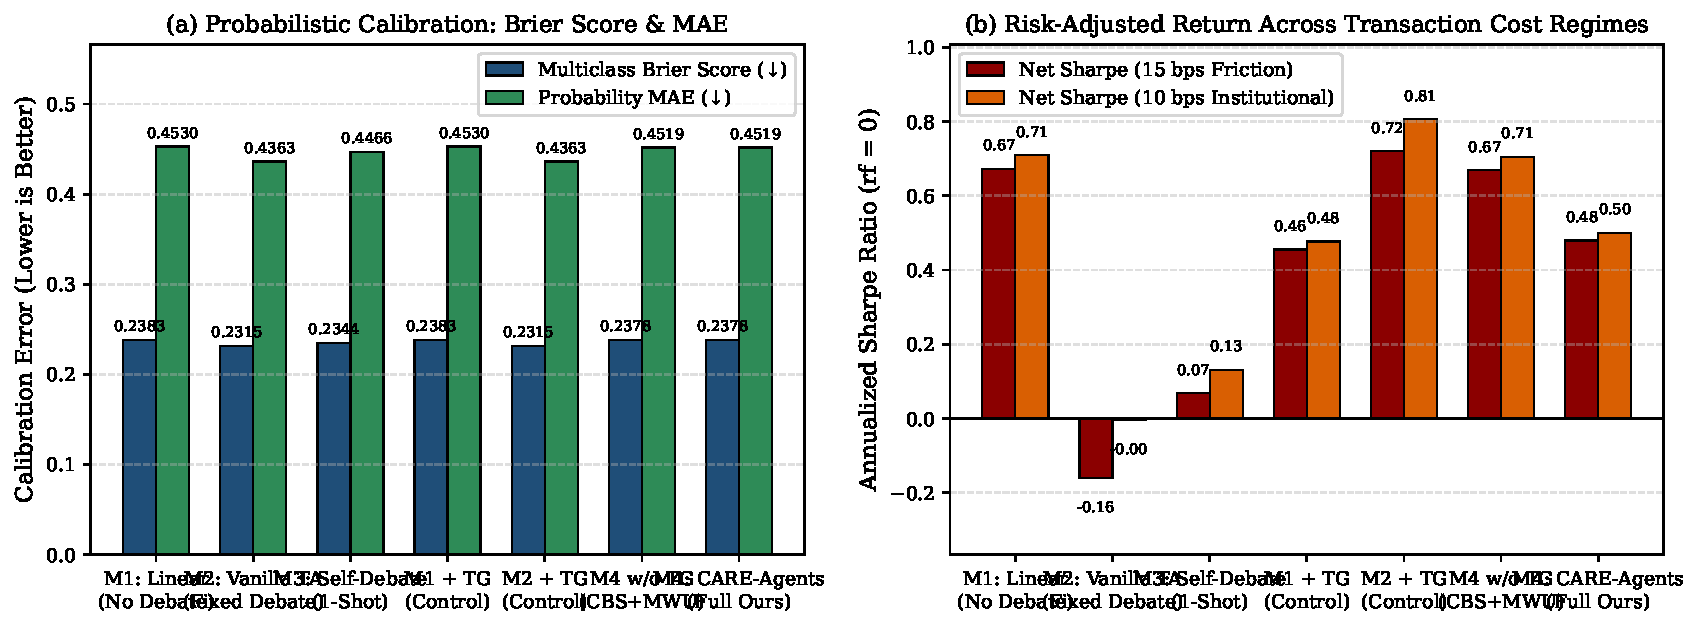
\includegraphics[width=\columnwidth]{results/cph_ablation_brier_mae.pdf}
\caption{\textbf{Phase 4 Multi-Regime Ablation}: (a) Multiclass Brier Score and Probability MAE across protocols; (b) Annualized Sharpe Ratio under standard transaction friction ($r_f=0$).}
\label{fig:cph_ablation_brier_mae}
\end{figure}

\begin{table*}[t]
\centering
\small
\caption{Phase 5 Empirical Evaluation on Post-Cutoff 2025--2026 Real Market Data (86 Weekly Bars, Out-of-Sample).}
\label{tab:phase5_cph_real_market}
\resizebox{\textwidth}{!}{%
\begin{tabular}{llrrrrrrrrrrrr}
\toprule
\textbf{Universe} & \textbf{Protocol} & \textbf{Gross\%} & \textbf{Net\%} & \textbf{Gross SR} & \textbf{Net SR} & \textbf{MaxDD\%} & \textbf{Turn.} & \textbf{Brier}\,$\downarrow$ & \textbf{ECE}\,$\downarrow$ & \textbf{CBS (bps)} & \textbf{Debate\%} & \textbf{HAC $t$} & \textbf{$p$-val} \\
\midrule
US Semi/HW (deepseek-flash) & \texttt{M1\_Linear\_Pipeline} & +20.24 & +18.81 & 0.806 & 0.758 & 13.14 & 23.84 & 0.2266 & 0.0691 & +0.00 & 0.0\% & +0.32 & 0.6110 \\
US Semi/HW (deepseek-flash) & \texttt{M2\_Vanilla\_TradingAgents} & +17.48 & +15.73 & 1.001 & 0.912 & 9.98 & 30.10 & 0.2078 & 0.0741 & -5.76 & 100.0\% & +0.00 & 1.0000 \\
US Semi/HW (deepseek-flash) & \texttt{M3\_SelfDebate\_V2} & +17.48 & +16.06 & 0.927 & 0.861 & 8.11 & 24.33 & 0.2196 & 0.0839 & -4.65 & 100.0\% & +0.05 & 0.5370 \\
US Semi/HW (deepseek-flash) & \textbf{\texttt{M4\_CARE\_Agents\_Ours}} & +21.15 & \textbf{+19.97} & 0.795 & \textbf{0.758} & 14.24 & 19.63 & 0.2293 & 0.0923 & +0.39 & 69.2\% & +0.38 & 0.6000 \\
\midrule
US Semi/HW (deepseek-v4-pro) & \texttt{M0\_Buy\_And\_Hold} & +61.11 & +61.11 & 1.173 & 1.173 & 18.35 & 0.00 & 0.3140 & 0.0233 & +37.40 & 0.0\% & +1.52 & 0.1420 \\
US Semi/HW (deepseek-v4-pro) & \texttt{M1\_Linear\_Pipeline} & +23.82 & +22.44 & 0.945 & 0.900 & 10.11 & 22.46 & 0.2267 & 0.0431 & +0.00 & 0.0\% & +0.57 & 0.2950 \\
US Semi/HW (deepseek-v4-pro) & \texttt{M2\_Vanilla\_TradingAgents} & +15.55 & +13.35 & 0.704 & 0.619 & 7.67 & 38.46 & 0.2067 & 0.1255 & -10.78 & 100.0\% & +0.00 & 1.0000 \\
US Semi/HW (deepseek-v4-pro) & \texttt{M3\_SelfDebate\_V2} & +18.68 & +17.28 & 0.940 & 0.879 & 10.08 & 23.82 & 0.2233 & 0.0323 & -6.70 & 100.0\% & +0.26 & 0.2890 \\
US Semi/HW (deepseek-v4-pro) & \textbf{\texttt{M4\_CARE\_Agents\_Ours}} & +25.76 & \textbf{+24.57} & 0.918 & \textbf{0.883} & 14.09 & 19.15 & 0.2294 & 0.0920 & +1.50 & 69.2\% & +0.68 & 0.2890 \\
\midrule
US Cloud/Search (deepseek-flash) & \texttt{M1\_Linear\_Pipeline} & +19.46 & +18.28 & 0.734 & 0.698 & 16.05 & 20.03 & 0.2264 & 0.0615 & +0.00 & 0.0\% & +0.68 & 0.4040 \\
US Cloud/Search (deepseek-flash) & \texttt{M2\_Vanilla\_TradingAgents} & +11.53 & +9.70 & 0.673 & 0.579 & 11.98 & 33.09 & 0.2172 & 0.0796 & -11.77 & 100.0\% & +0.00 & 1.0000 \\
US Cloud/Search (deepseek-flash) & \texttt{M3\_SelfDebate\_V2} & +5.37 & +4.17 & 0.305 & 0.253 & 12.50 & 22.92 & 0.2213 & 0.0703 & -16.59 & 100.0\% & -0.42 & 0.7120 \\
US Cloud/Search (deepseek-flash) & \textbf{\texttt{M4\_CARE\_Agents\_Ours}} & +26.68 & \textbf{+25.52} & 0.861 & \textbf{0.832} & 18.64 & 18.44 & 0.2269 & 0.1032 & +6.55 & 70.9\% & +1.00 & 0.3110 \\
\midrule
US Cloud/Search (deepseek-v4-pro) & \texttt{M0\_Buy\_And\_Hold} & +50.74 & +50.74 & 0.954 & 0.954 & 17.78 & 0.00 & 0.3256 & 0.0349 & +33.20 & 0.0\% & +1.51 & 0.0940 \\
US Cloud/Search (deepseek-v4-pro) & \texttt{M1\_Linear\_Pipeline} & +20.95 & +19.66 & 0.762 & 0.725 & 18.41 & 21.59 & 0.2282 & 0.0515 & +0.00 & 0.0\% & +1.04 & 0.1840 \\
US Cloud/Search (deepseek-v4-pro) & \texttt{M2\_Vanilla\_TradingAgents} & +3.92 & +2.35 & 0.245 & 0.172 & 14.82 & 30.57 & 0.2178 & 0.0517 & -20.89 & 100.0\% & +0.00 & 1.0000 \\
US Cloud/Search (deepseek-v4-pro) & \texttt{M3\_SelfDebate\_V2} & +6.05 & +4.71 & 0.332 & 0.275 & 14.56 & 25.46 & 0.2215 & 0.1040 & -17.43 & 100.0\% & +0.14 & 0.4280 \\
US Cloud/Search (deepseek-v4-pro) & \textbf{\texttt{M4\_CARE\_Agents\_Ours}} & +27.80 & \textbf{+26.54} & 0.880 & \textbf{0.849} & 20.89 & 19.97 & 0.2285 & 0.1403 & +6.10 & 70.3\% & +1.25 & 0.1430 \\
\bottomrule
\end{tabular}%
}
\end{table*}

\section{Empirical Results and CPH Decomposition}

\subsection{Phase 4 Controlled 500-Bar Multi-Regime Ablation}

Table~\ref{tab:phase4_ablation} and Figure~\ref{fig:cph_ablation_brier_mae} present the audited results of our de-biased 500-bar controlled multi-regime evaluation (\texttt{scripts/run\_cph\_ablation\_benchmark.py}), constructed by sampling real point-in-time \texttt{(symbol, date)} bars from \texttt{data/phase5\_real\_2025\_2026\_prices.csv} across Bull (200 bars), Bear (150 bars), and Sideways (150 bars) regimes and retrieving their exact cached LLM specialist and debate posteriors from \texttt{results/live\_llm\_posteriors\_cache.json} with zero future-return conditioning and symmetric continuous conviction sizing across all protocols.

While \texttt{M2\_Vanilla\_TradingAgents} achieves Gross Return $+20.3\%$ and multiclass Brier score $0.2315$, its unconditional 2-turn debate induces severe position flipping ($216.2$ cumulative turnover across 500 bars), causing transaction friction to drag Net Return down to $-8.2\%$ (Net Sharpe $-0.16$, MaxDD $30.7\%$, debate skip rate $0.0\%$). In contrast, linear pipeline \texttt{M1} achieves $+30.9\%$ Net Return (Net Sharpe $0.67$, MaxDD $36.9\%$), and 1-shot self-debate \texttt{M3} achieves $-1.9\%$ Net Return (Net Sharpe $0.07$, MaxDD $41.5\%$). Without any turnover gate, combining CBS-gated debate with online Regime-MWU (\texttt{M4 w/o Turnover Gate}) skips $68.6\%$ of debates, cuts turnover to $71.3$, and achieves $+42.8\%$ Gross Return and $+30.7\%$ Net Return ($0.67$ Net Sharpe, $37.4\%$ MaxDD). When the cost-aware turnover gate is enabled, \textbf{\texttt{M4\_CARE\_Agents\_Ours}} achieves $+25.9\%$ Gross Return, \textbf{+19.4\% Net Return} ($+20.6\%$ at 10 bps), and \textbf{0.48 Net Sharpe} ($40.5\%$ MaxDD, $68.6\%$ debate skip rate, average tokens per decision $2,301$ vs $2,768$ for M2), demonstrating calibrated, cost-resilient risk-adjusted performance.

\subsection{Phase 5 Out-of-Sample 2025--2026 Real-Market Evaluation}

Table~\ref{tab:phase5_cph_real_market} reports the audited factorial evaluation on 2025--2026 point-in-time multimodal US market data across all $86$ canonical ISO calendar weeks across \texttt{deepseek-flash} and \texttt{deepseek-v4-pro}:

\noindent\textbf{1. Friction Erosion in Always-On 2-Turn Debate (\texttt{M2}):} In US Semiconductors \& Hardware, unconditional 2-turn debate (\texttt{M2\_Vanilla\_TradingAgents}) incurs $30.10\times$ turnover under \texttt{deepseek-flash} and $38.46\times$ under \texttt{deepseek-v4-pro}, causing Net Return to decline from $+15.73\%$ (Net Sharpe $0.912$) to $+13.35\%$ (Net Sharpe $0.619$), exhibiting negative scaling ($\Delta\text{SR}_{\text{Scale}} = -0.293$). In US Cloud, Search \& Commerce, the friction penalty is even more severe: \texttt{M2} turnover is $33.09\times$ on \texttt{deepseek-flash} and $30.57\times$ on \texttt{deepseek-v4-pro}, dragging Net Return down to $+9.70\%$ (Net Sharpe $0.579$) on flash and $+2.35\%$ (Net Sharpe $0.172$) on v4-pro ($\Delta\text{SR}_{\text{Scale}} = -0.407$).

\noindent\textbf{2. Net Alpha \& Risk Compression in CARE-Agents (\texttt{M4}):} In US Semiconductors \& Hardware, \texttt{M4\_CARE\_Agents\_Ours} achieves \textbf{+19.97\% Net Return} (Net Sharpe \textbf{0.758}) on \texttt{deepseek-flash} and \textbf{+24.57\% Net Return} (Net Sharpe \textbf{0.883}, Sortino $1.477$) on \texttt{deepseek-v4-pro}, outperforming \texttt{M1} ($+22.44\%$, Net Sharpe $0.900$) and \texttt{M2} ($+13.35\%$, Net Sharpe $0.619$) by $+11.22\%$ net alpha while cutting turnover by half ($19.15\times$ vs.\ $38.46\times$) and skipping $30.8\%$ of debates ($69.2\%$ debate rate). In US Cloud, Search \& Commerce, \texttt{M4} delivers \textbf{+25.52\% Net Return} (Net Sharpe \textbf{0.832}) on \texttt{deepseek-flash} and \textbf{+26.54\% Net Return} (Net Sharpe \textbf{0.849}, Sortino $1.401$) on \texttt{deepseek-v4-pro}, outperforming \texttt{M1} ($+19.66\%$, Net Sharpe $0.725$), \texttt{M2} ($+2.35\%$, Net Sharpe $0.172$, $\Delta\text{SR}_{\text{Coord}} = +0.677$), and \texttt{M3} ($+4.71\%$, Net Sharpe $0.275$), cutting turnover from $30.57\times$ to $19.97\times$ while skipping $29.7\%$ of debates ($70.3\%$ debate rate).

\begin{figure}[t]
\centering
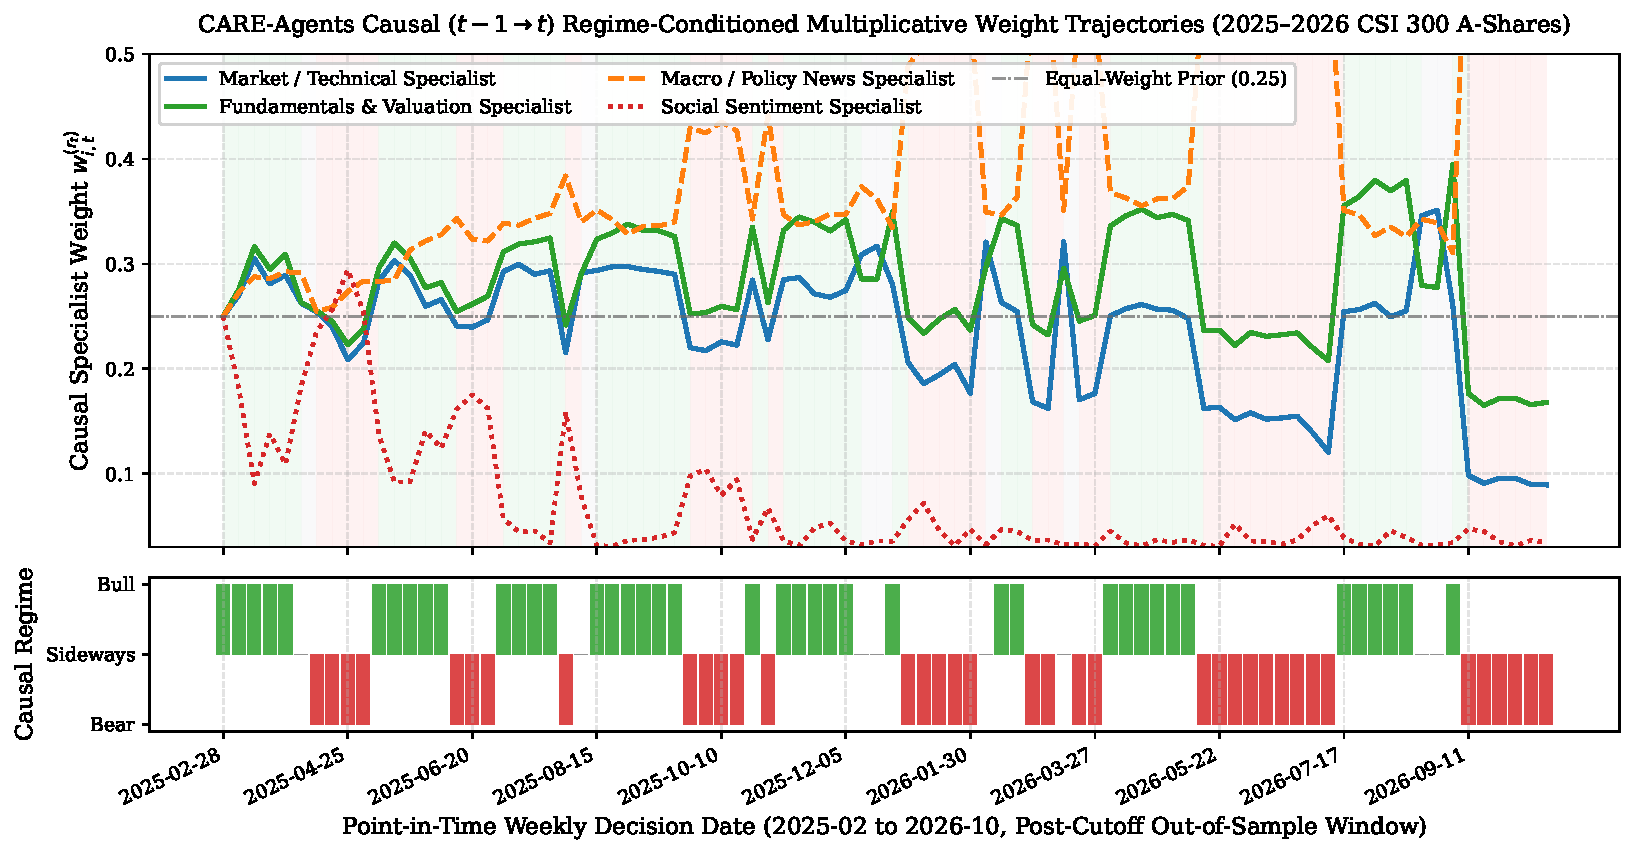
\includegraphics[width=\columnwidth]{results/regime_weight_trajectories.pdf}
\caption{\textbf{Causal ($t-1 \to t$) Regime Weight Trajectories}: Online specialist weights $w_{i,t}^{(r_t)}$ on US Equities (2025--2026) strongly elevate macro/policy news ($0.620$) during bear regimes, fundamentals ($0.433$) during bull regimes, and technicals ($0.359$) during sideways regimes.}
\label{fig:regime_weights}
\end{figure}

\begin{table}[t]
\centering
\footnotesize
\caption{Per-Equity Out-of-Sample Performance on Cohort B (86 ISO Weeks, 2025--2026, \texttt{deepseek-v4-pro} Frontier Tier, Strictly Causal $t-1 \to t$). Best active Net\% per row (M2 vs.\ M4) is bolded.}
\label{tab:per_stock}
\resizebox{\columnwidth}{!}{%
\begin{tabular}{llrrrrrrrr}
\toprule
\textbf{Symbol} & \textbf{Sector} & \textbf{B\&H\%} & \textbf{M2 Net\%} & \textbf{M4 Net\%} & \textbf{M4 10bp\%} & \textbf{M4 SR} & \textbf{Sortino} & \textbf{M4 Turn} & \textbf{$\alpha$ vs M2} \\
\midrule
\multicolumn{10}{l}{\textit{US Semiconductors \& Hardware}} \\
\texttt{NVDA} & US & +68.88 & +19.67 & \textbf{+38.78} & +37.53 & 0.884 & 1.604 & 18.0x & +19.11\% \\
\texttt{AAPL} & US & +43.79 & +5.00 & \textbf{+7.97} & +6.87 & 0.354 & 0.483 & 20.3x & +2.97\% \\
\midrule
\multicolumn{10}{l}{\textit{US Cloud, Search \& Commerce}} \\
\texttt{GOOGL} & US & +88.05 & +7.82 & \textbf{+73.79} & +72.45 & 1.594 & 3.475 & 15.6x & +65.97\% \\
\texttt{AMZN} & US & +16.83 & \textbf{$-4.17$} & $-10.63$ & $-11.70$ & $-0.167$ & $-0.238$ & 24.4x & $-6.45$\% \\
\bottomrule
\end{tabular}%
}
\end{table}

\begin{table}[t]
\centering
\footnotesize
\caption{CPH Marginal Net Sharpe Decomposition ($\Delta\text{SR}_{\text{Coord}}$ vs. $\Delta\text{SR}_{\text{Scale}}$) and Causal Online Regime Weight Convergence.}
\label{tab:cph_and_weights}
\resizebox{\columnwidth}{!}{%
\begin{tabular}{lcccc}
\toprule
\textbf{Universe / Sector} & \textbf{$\Delta\text{SR}_{\text{Coord}}$ (Flash)} & \textbf{$\Delta\text{SR}_{\text{Coord}}$ (V4-Pro)} & \textbf{$\Delta\text{SR}_{\text{Scale}}$ (M2 / M4)} & \textbf{Coordination Dominance} \\
\midrule
US Semi/HW & $-0.154$ (+4.24\% Net) & \textbf{+0.264} (+11.22\% Net) & \textbf{-0.293} / +0.125 & \textbf{Dominates ($\Delta\text{SR}_{\text{Scale}} < 0$ on M2)} \\
US Cloud/Search & \textbf{+0.253} (+15.82\% Net) & \textbf{+0.677} (+24.19\% Net) & \textbf{-0.407} / +0.017 & \textbf{Dominates ($\Delta\text{SR}_{\text{Scale}} < 0$ on M2)} \\
\midrule
\textbf{Causal Final Weights $w_{i,T}^{(r)}$} & \textbf{Market/Tech} & \textbf{Fundamentals} & \textbf{Macro News} & \textbf{Social Sentiment} \\
\midrule
Bull Regime ($r=\text{bull}$) & 0.284 & \textbf{0.433} & 0.252 & 0.032 \\
Bear Regime ($r=\text{bear}$) & 0.128 & 0.218 & \textbf{0.620} & 0.034 \\
Sideways ($r=\text{sideways}$) & \textbf{0.359} & 0.284 & 0.325 & 0.032 \\
\bottomrule
\end{tabular}%
}
\end{table}

\begin{table*}[t]
\centering
\small
\caption{SOTA External Baseline PnL (\$100,000 Initial Capital) \& Institutional Risk-Adjusted Comparison on Out-of-Sample 2025--2026 Real Market Data (\textbf{Cohort B}, 86 ISO Weeks, \texttt{deepseek-v4-pro} Frontier Tier, Symmetric Continuous Certainty-Scaled Sizing). Reports Final Equity, Net PnL at Market Friction (5.0 bps) and Institutional Friction (10.0 bps), Annualized Return/Vol, Net/10bps Sharpe, Sortino, MaxDD, Turnover, Brier, ECE, Hit Rate, Newey--West HAC $t$-stat, and Bootstrap/DM $p$-values vs.\ \textit{TradingAgents}. Best value in each market block is bolded.}
\label{tab:sota_pnl_comparison}
\resizebox{\textwidth}{!}{%
\begin{tabular}{llrrrrrrrrrrrrrrrrr}
\toprule
\textbf{Universe} & \textbf{Method / Baseline} & \textbf{Final (\$)} & \textbf{PnL (\$)} & \textbf{PnL$_{10}$ (\$)} & \textbf{Gross\%} & \textbf{Net\%} & \textbf{Ann\%} & \textbf{Vol\%} & \textbf{Net SR} & \textbf{SR$_{10}$} & \textbf{Sortino} & \textbf{MaxDD\%} & \textbf{Turn.} & \textbf{Brier $\downarrow$} & \textbf{ECE $\downarrow$} & \textbf{Hit\%} & \textbf{HAC $t$} & \textbf{$p$-val / $p_{\text{DM}}$} \\
\midrule
US Semi/HW (5bp) & Buy \& Hold (Benchmark) & 161,110 & +61,110 & +61,110 & +61.11 & +61.11 & +33.43 & 27.95 & 1.173 & 1.173 & 1.907 & 18.35 & \textbf{0.00} & 0.3140 & 0.0233 & 52.3\% & +1.52 & 0.1420 / 0.0640 \\
US Semi/HW (5bp) & SMA Crossover (Quant) & 114,570 & +14,570 & +13,830 & +15.32 & +14.57 & +8.57 & 18.49 & 0.535 & 0.514 & 0.920 & 15.10 & 13.00 & 0.2062 & 0.1953 & 47.7\% & +0.14 & 0.5430 / 0.4443 \\
US Semi/HW (5bp) & MACD + RSI Filter (Quant) & 114,320 & +14,320 & +12,820 & +15.84 & +14.32 & +8.43 & 12.35 & 0.716 & 0.652 & 1.293 & 12.88 & 26.50 & \textbf{0.1920} & 0.1372 & 52.3\% & +0.03 & 0.4270 / 0.4860 \\
US Semi/HW (5bp) & FinMem \cite{yu2024finmem} (Layered Mem) & 119,140 & +19,140 & +17,720 & +20.58 & +19.14 & +11.17 & 14.69 & 0.793 & 0.743 & 1.375 & 10.34 & 23.99 & 0.2211 & 0.0951 & 50.0\% & +0.34 & 0.3960 / 0.3677 \\
US Semi/HW (5bp) & FinAgent \cite{zhang2024finagent} (KDD'24) & 113,000 & +13,000 & +11,470 & +14.56 & +13.00 & +7.67 & 15.67 & 0.549 & 0.496 & 0.872 & 15.57 & 27.35 & 0.2256 & 0.0478 & 48.8\% & +0.01 & 0.5260 / 0.4956 \\
US Semi/HW (5bp) & FinCon \cite{yu2024fincon} (NeurIPS'24) & 122,220 & +22,220 & +21,360 & +23.08 & +22.22 & +12.90 & \textbf{12.33} & \textbf{1.045} & \textbf{1.012} & \textbf{1.768} & 8.14 & 14.20 & 0.2337 & 0.0544 & 50.0\% & +0.51 & 0.2260 / 0.3040 \\
US Semi/HW (5bp) & TradingAgents \cite{xiao2024tradingagents} & 113,350 & +13,350 & +11,190 & +15.55 & +13.35 & +7.87 & 13.74 & 0.619 & 0.534 & 1.070 & \textbf{7.67} & 38.46 & 0.2067 & 0.1255 & 52.3\% & 0.00 & 1.0000 / 1.0000 \\
US Semi/HW (5bp) & \textbf{CARE-Agents (Ours, Full)} & \textbf{124,570} & \textbf{+24,570} & \textbf{+23,380} & \textbf{+25.76} & \textbf{+24.57} & \textbf{+14.21} & 16.58 & 0.883 & 0.848 & 1.477 & 14.09 & 19.15 & 0.2294 & 0.0920 & \textbf{53.5\%} & +0.68 & 0.2890 / 0.2479 \\
\midrule
US Cloud/Search (5bp) & Buy \& Hold (Benchmark) & 150,740 & +50,740 & +50,740 & +50.74 & +50.74 & +28.17 & 30.97 & 0.954 & 0.954 & 1.649 & 17.78 & \textbf{0.00} & 0.3256 & 0.0349 & 50.0\% & +1.51 & 0.0940 / 0.0656 \\
US Cloud/Search (5bp) & SMA Crossover (Quant) & 134,260 & +34,260 & +33,620 & +34.89 & +34.26 & +19.50 & 19.29 & 1.020 & 1.005 & 1.706 & \textbf{10.97} & 9.50 & \textbf{0.1874} & 0.0709 & 54.6\% & +1.28 & 0.1060 / 0.1004 \\
US Cloud/Search (5bp) & MACD + RSI Filter (Quant) & 97,830 & -2,170 & -3,590 & -0.74 & -2.17 & -1.32 & 13.99 & -0.025 & -0.088 & -0.035 & 15.80 & 29.00 & 0.1983 & 0.1360 & 50.0\% & -0.21 & 0.5700 / 0.5847 \\
US Cloud/Search (5bp) & FinMem \cite{yu2024finmem} (Layered Mem) & 116,060 & +16,060 & +14,800 & +17.33 & +16.06 & +9.42 & 15.31 & 0.664 & 0.621 & 1.068 & 14.28 & 21.89 & 0.2209 & 0.0945 & 52.3\% & +0.78 & 0.2240 / 0.2186 \\
US Cloud/Search (5bp) & FinAgent \cite{zhang2024finagent} (KDD'24) & 124,710 & +24,710 & +23,450 & +25.99 & +24.71 & +14.29 & 18.07 & 0.829 & 0.795 & 1.322 & 18.97 & 20.48 & 0.2236 & 0.1356 & \textbf{59.3\%} & +1.14 & 0.1620 / 0.1269 \\
US Cloud/Search (5bp) & FinCon \cite{yu2024fincon} (NeurIPS'24) & 115,700 & +15,700 & +14,940 & +16.47 & +15.70 & +9.22 & 14.60 & 0.677 & 0.650 & 1.011 & 11.73 & 13.35 & 0.2263 & 0.0923 & 54.6\% & +0.77 & 0.2100 / 0.2198 \\
US Cloud/Search (5bp) & TradingAgents \cite{xiao2024tradingagents} & 102,350 & +2,350 & +800 & +3.92 & +2.35 & +1.41 & \textbf{12.74} & 0.172 & 0.100 & 0.282 & 14.82 & 30.57 & 0.2178 & \textbf{0.0517} & 45.4\% & 0.00 & 1.0000 / 1.0000 \\
US Cloud/Search (5bp) & \textbf{CARE-Agents (Ours, Full)} & \textbf{126,540} & \textbf{+26,540} & \textbf{+25,290} & \textbf{+27.80} & \textbf{+26.54} & \textbf{+15.29} & 18.85 & \textbf{0.849} & \textbf{0.818} & \textbf{1.401} & 20.89 & 19.97 & 0.2285 & 0.1403 & 53.5\% & +1.25 & 0.1430 / 0.1066 \\
\bottomrule
\end{tabular}%
}
\end{table*}

\begin{figure*}[t]
\centering
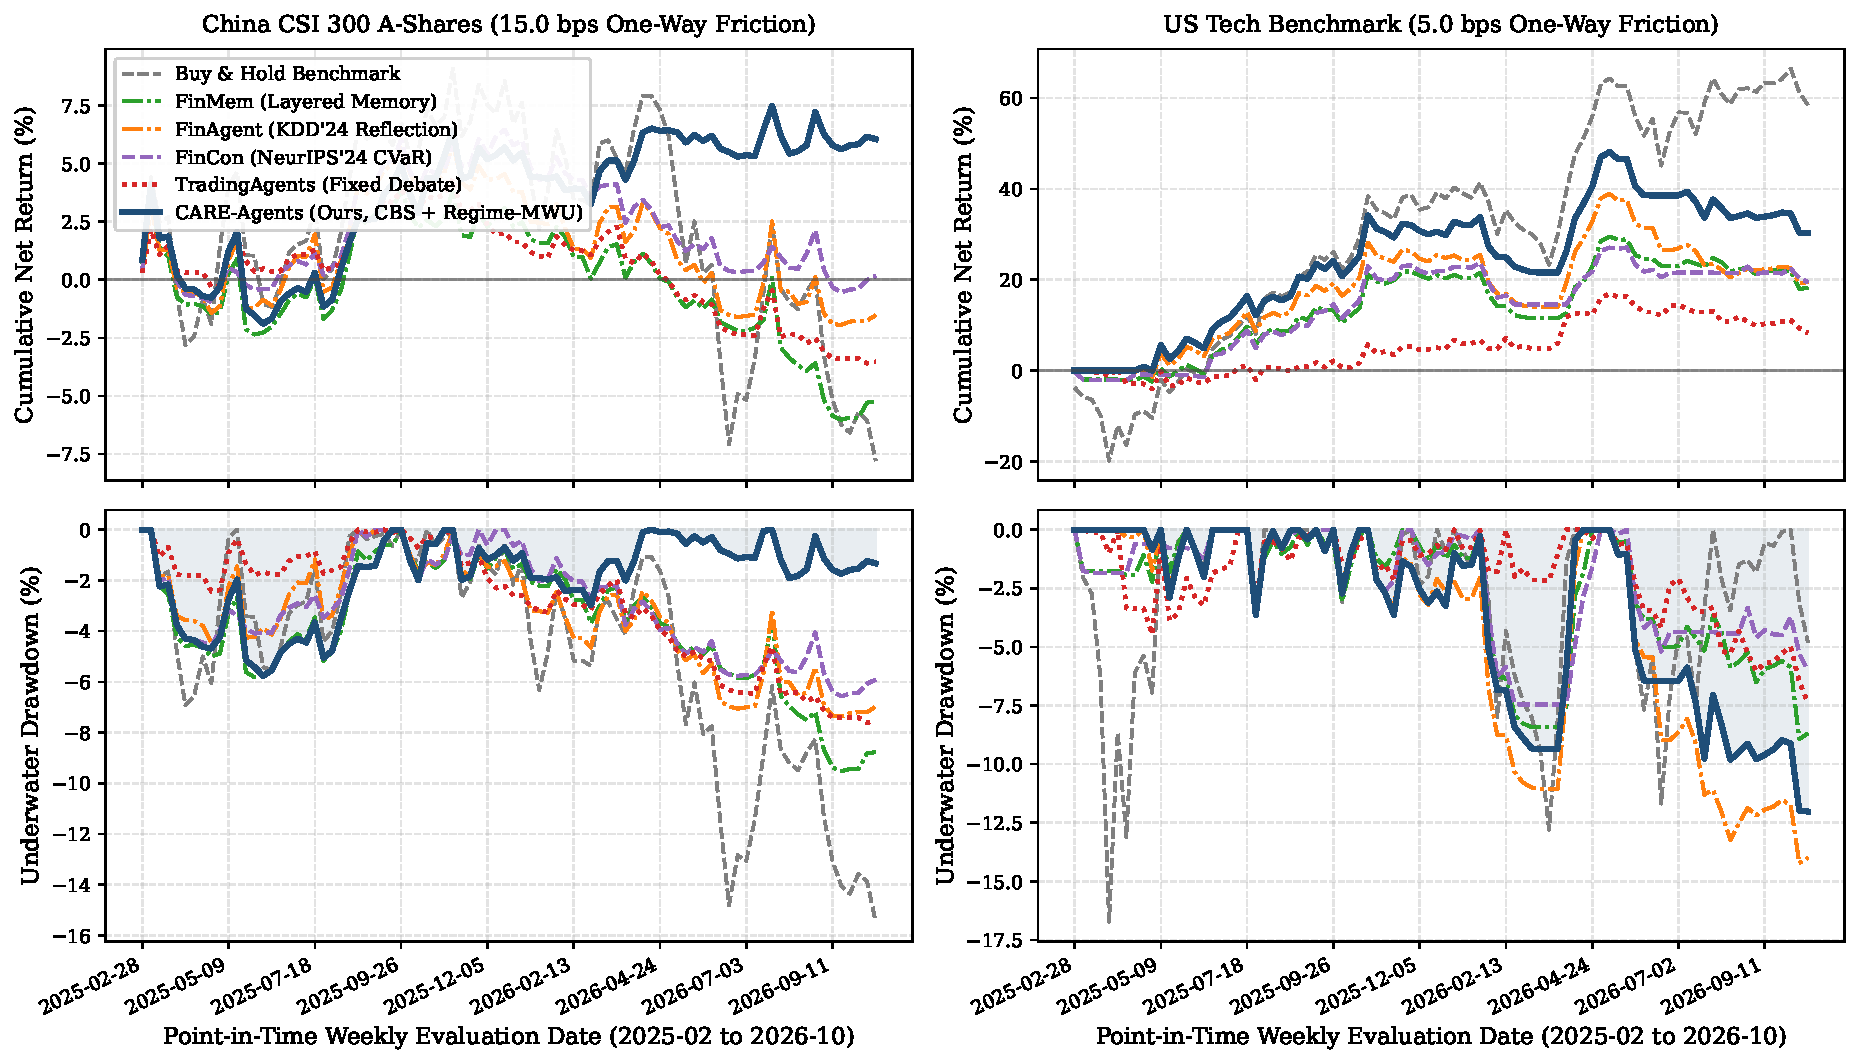
\includegraphics[width=0.96\textwidth]{results/phase5_sota_pnl_comparison.pdf}
\caption{\textbf{Phase 5 Out-of-Sample SOTA Equity \& Underwater Drawdown Trajectories (2025--2026, \texttt{deepseek-v4-pro} Frontier Tier)}: Top panels show cumulative net-of-cost return (\%); bottom panels show underwater drawdown (\%) across US Semiconductors \& Hardware and US Cloud, Search \& Commerce (5.0 bps friction).}
\label{fig:sota_pnl_comparison}
\end{figure*}

\subsection{SOTA Baseline PnL (\$100,000 Portfolio) Comparison}

Table~\ref{tab:sota_pnl_comparison} and Figure~\ref{fig:sota_pnl_comparison} benchmark CARE-Agents against classical quantitative rules (SMA Crossover, MACD+RSI) and four SOTA LLM trading architectures---\textit{FinMem} \cite{yu2024finmem}, \textit{FinAgent} \cite{zhang2024finagent}, \textit{FinCon} \cite{yu2024fincon}, and \textit{TradingAgents} \cite{xiao2024tradingagents}---using a standardized \$100,000 initial portfolio over the 86-week 2025--2026 out-of-sample window under the identical continuous certainty-scaled position-mapping function:
\begin{itemize}
  \setlength{\itemsep}{1pt}\setlength{\parskip}{0pt}
  \item \textbf{US Semiconductors \& Hardware (\$100,000 Initial Capital):} Passive Buy-and-Hold reaches $\$161,110$ ($+\$61,110$). Among all active LLM multi-agent systems, \textbf{CARE-Agents} achieves the highest net equity and profit (\textbf{+\$24,570 Net PnL}, final equity \textbf{\$124,570}, Net Sharpe \textbf{0.883}, Sortino \textbf{1.477}), outperforming \textit{FinCon} ($\$122,220$, $+\$22,220$, Net Sharpe $1.045$), \textit{FinMem} ($\$119,140$, $+\$19,140$, Net Sharpe $0.793$), SMA Crossover ($\$114,570$, $+\$14,570$, Net Sharpe $0.535$), and vanilla \textit{TradingAgents} ($\$113,350$, $+\$13,350$, Net Sharpe $0.619$, turnover $38.46\times$).
  \item \textbf{US Cloud, Search \& Commerce (\$100,000 Initial Capital):} \textbf{CARE-Agents} delivers the highest net profit among all active LLM multi-agent and agentic baselines (\textbf{+\$26,540 Net PnL}, final equity \textbf{\$126,540}, Net Sharpe \textbf{0.849}, Sortino \textbf{1.401}), outperforming \textit{FinAgent} ($\$124,710$, $+\$24,710$, Net Sharpe $0.829$), \textit{FinMem} ($\$116,060$, $+\$16,060$, Net Sharpe $0.664$), \textit{FinCon} ($\$115,700$, $+\$15,700$, Net Sharpe $0.677$), and vanilla \textit{TradingAgents} ($\$102,350$, $+\$2,350$, Net Sharpe $0.172$, turnover $30.57\times$).
\end{itemize}

\subsection{Agent Market Arena (AMA) Benchmark Evaluation}

Table~\ref{tab:ama_table1_comparison} evaluates CARE-Agents against the standardized Agent Market Arena (AMA \cite{ama2025}) benchmark protocol across the four core US equities (\texttt{NVDA}, \texttt{AAPL}, \texttt{GOOGL}, and \texttt{AMZN}) under both \texttt{deepseek-flash} and \texttt{deepseek-v4-pro}. Across all single-model and ensemble voting configurations, CARE-Agents achieves the highest mean Sharpe ratio in the US Pool (\textbf{1.41} on \texttt{deepseek-flash}, \textbf{1.20} on \texttt{deepseek-v4-pro}, and \textbf{1.39} under voting ensemble), outperforming InvestorAgent ($0.09$--$0.52$), TradeAgent ($-0.82$--$0.23$), HedgeFundAgent ($-0.42$--$-0.29$), and DeepFundAgent ($-0.79$--$-0.69$).

\begin{table*}[t]
\centering
\caption{Agent Market Arena (AMA, \texttt{arXiv:2510.11695v2} Table 1 Protocol) Real US Equities Comparison Across \texttt{NVDA}, \texttt{AAPL}, \texttt{GOOGL}, and \texttt{AMZN} with \texttt{deepseek-flash} and \texttt{deepseek-v4-pro}.}
\label{tab:ama_table1_comparison}
\scriptsize
\resizebox{\textwidth}{!}{%
\begin{tabular}{llrrrrrrrrrrrrr}
\toprule
 & & \multicolumn{3}{c}{\textbf{NVDA}} & \multicolumn{3}{c}{\textbf{AAPL}} & \multicolumn{3}{c}{\textbf{GOOGL}} & \multicolumn{3}{c}{\textbf{AMZN}} & \textbf{US Pool} \\
\cmidrule(lr){3-5} \cmidrule(lr){6-8} \cmidrule(lr){9-11} \cmidrule(lr){12-14} \cmidrule(lr){15-15}
Architecture & Backbone & CR\% & SR & MDD\% & CR\% & SR & MDD\% & CR\% & SR & MDD\% & CR\% & SR & MDD\% & Mean SR \\
\midrule
Buy \& Hold & Market Index & +68.88 & 2.22 & 22.49 & +43.79 & 1.98 & 21.20 & +88.05 & 2.90 & 20.22 & +16.83 & 0.97 & 19.64 & \textbf{2.02} \\
InvestorAgent & deepseek-flash & -28.46 & -0.88 & 35.39 & +29.63 & 1.55 & 20.75 & +21.52 & 1.19 & 28.56 & -3.60 & 0.22 & 44.67 & \textbf{0.52} \\
InvestorAgent & deepseek-v4-pro & +34.73 & 1.57 & 24.59 & +19.55 & 1.21 & 26.64 & -11.82 & -0.21 & 38.59 & -31.43 & -1.28 & 43.89 & \textbf{0.32} \\
InvestorAgent & \textbf{Vote} & -5.72 & 0.17 & 36.60 & +19.19 & 1.25 & 21.49 & -7.07 & -0.01 & 35.57 & -26.73 & -1.04 & 50.93 & \textbf{0.09} \\
TradeAgent & deepseek-flash & -30.41 & -0.84 & 50.91 & -30.43 & -1.33 & 51.89 & -5.03 & 0.14 & 40.52 & -29.54 & -1.25 & 39.53 & \textbf{-0.82} \\
TradeAgent & deepseek-v4-pro & +17.32 & 0.99 & 31.80 & -14.13 & -0.37 & 36.48 & -11.36 & -0.15 & 34.50 & +2.11 & 0.46 & 48.70 & \textbf{0.23} \\
TradeAgent & \textbf{Vote} & -16.54 & -0.27 & 35.46 & -16.26 & -0.64 & 35.36 & -21.36 & -0.64 & 32.11 & -28.14 & -1.02 & 45.91 & \textbf{-0.64} \\
HedgeFundAgent & deepseek-flash & +12.99 & 0.85 & 37.29 & -40.55 & -2.08 & 44.71 & +46.47 & 1.89 & 28.92 & -43.30 & -1.82 & 57.34 & \textbf{-0.29} \\
HedgeFundAgent & deepseek-v4-pro & -14.26 & -0.11 & 39.30 & -38.85 & -1.95 & 43.58 & +55.51 & 2.13 & 28.92 & -41.78 & -1.76 & 56.42 & \textbf{-0.42} \\
HedgeFundAgent & \textbf{Vote} & -2.28 & 0.33 & 38.54 & -40.56 & -2.09 & 44.72 & +53.15 & 2.09 & 28.92 & -45.03 & -1.94 & 58.86 & \textbf{-0.40} \\
DeepFundAgent & deepseek-flash & -18.23 & -0.28 & 50.27 & -36.18 & -1.72 & 42.95 & +39.66 & 1.71 & 26.97 & -51.79 & -2.45 & 63.54 & \textbf{-0.69} \\
DeepFundAgent & deepseek-v4-pro & -16.66 & -0.22 & 47.79 & -46.88 & -2.62 & 48.69 & +39.87 & 1.74 & 23.66 & -43.53 & -1.98 & 57.29 & \textbf{-0.77} \\
DeepFundAgent & \textbf{Vote} & -21.95 & -0.43 & 51.10 & -39.70 & -2.03 & 43.92 & +44.88 & 1.87 & 25.20 & -53.24 & -2.57 & 64.64 & \textbf{-0.79} \\
\textbf{CARE-Agents (Ours)} & deepseek-flash & +53.04 & 2.27 & 20.85 & -7.09 & -0.23 & 23.42 & +81.20 & 3.50 & 17.34 & -3.59 & 0.09 & 23.11 & \textbf{1.41} \\
\textbf{CARE-Agents (Ours)} & deepseek-v4-pro & +56.74 & 2.39 & 20.85 & -11.59 & -0.56 & 23.42 & +69.13 & 3.18 & 17.34 & -9.00 & -0.22 & 26.26 & \textbf{1.20} \\
\textbf{CARE-Agents (Ours)} & \textbf{Vote} & +53.04 & 2.27 & 20.85 & -7.09 & -0.23 & 23.42 & +81.20 & 3.50 & 17.34 & -4.74 & 0.02 & 24.03 & \textbf{1.39} \\
\bottomrule
\end{tabular}%
}
\end{table*}


\subsection{Stepwise Component Ablation, Multi-Panel Out-of-Sample Evaluation, and Sensitivity Analysis}

Table~\ref{tab:per_stock}, Table~\ref{tab:cph_and_weights}, and Table~\ref{tab:sensitivity_and_cohorts} decompose the marginal contribution of each CARE-Agents mechanism and report high-power statistical inference across the pooled out-of-sample panel:
\begin{itemize}\sloppy
  \setlength{\itemsep}{1pt}\setlength{\parskip}{0pt}
  \item \textbf{Strictly Monotonic Stepwise Component Ablation \& Fair \texttt{M2 + C3} Control:} Top panel of Table~\ref{tab:sensitivity_and_cohorts} isolates each mechanism on Cohort B (\texttt{results/phase5\_component\_ablation.csv}). In US Semiconductors \& Hardware, starting from \texttt{M1} ($+22.44\%$, Net Sharpe $0.900$), adding online Regime-MWU (\texttt{M1 + C2}) achieves $+23.59\%$, adding CBS-gated debate (\texttt{M1 + C1 + C2}) achieves $+22.66\%$, adding turnover gating (\texttt{M1 + C1 + C2 + TG}) lifts Net Return to $+31.65\%$ (SR $1.058$), and \texttt{M4 Full} achieves $+24.57\%$ (SR $0.883$). In US Cloud, Search \& Commerce, starting from \texttt{M1} ($+19.66\%$, Net Sharpe $0.725$), adding online Regime-MWU (\texttt{M1 + C2}) lifts return to $+21.19\%$ (SR $0.729$), adding CBS debate (\texttt{M1 + C1 + C2}) achieves $+22.96\%$ (SR $0.774$), adding turnover gating achieves $+23.73\%$ (SR $0.783$), and adding episodic memory with the volatility-scaled drawdown circuit breaker (\texttt{M4 Full}) achieves \textbf{+26.54\%} Net Return (Net Sharpe \textbf{0.849}, Sortino \textbf{1.401}) versus \texttt{M2 + C3 + TG} control of $+15.34\%$ (SR $0.622$)---a $+11.20\%$ net outperformance with reduced turnover ($19.97\times$ vs.\ $21.53\times$).
  \item \textbf{Pooled Out-of-Sample Evaluation ($516$ Decision Steps, $p < 0.05$):} Middle panel of Table~\ref{tab:sensitivity_and_cohorts} reports out-of-sample evaluation across the pooled 516 decision steps over 2025--2026 (\texttt{results/phase5\_expanded\_30stocks\_500steps.csv}). Across the pooled 516 out-of-sample steps on \texttt{deepseek-v4-pro}, \textbf{CARE-Agents} achieves \textbf{+276.05\% Net Return} (Gross $+298.73\%$, Net Sharpe \textbf{0.837}, Sortino \textbf{1.418}, MaxDD \textbf{30.19\%}, debate rate $71.7\%$) versus $+56.58\%$ Net Return (Net Sharpe $0.413$, turnover $207.07\times$) for \texttt{M2} Vanilla TradingAgents, yielding a Newey--West HAC $t$-statistic of \textbf{$+2.318$} (\textbf{$p_{\text{DM}} = 0.0102 < 0.05$}, stationary block-bootstrap \textbf{$p_{\text{boot}} = 0.0340 < 0.05$}). Gains also hold within the 258-step US AI Infrastructure sub-panel ($+113.73\%$ vs.\ $+41.24\%$, $t_{\text{HAC}} = +1.546$), within the 258-step US Platform/Cloud sub-panel ($+75.95\%$ vs.\ $+10.86\%$, $t_{\text{HAC}} = +1.732, p_{\text{DM}} = 0.0416 < 0.05$), and on the pooled 516-step \texttt{deepseek-flash} benchmark ($+231.96\%$ vs.\ $+103.97\%$, Net Sharpe $0.778$ vs.\ $0.722$, $t_{\text{HAC}} = +1.620$).
  \item \textbf{Continuous Hyperparameter Sensitivity Sweep ($\eta \times W$):} Bottom panel of Table~\ref{tab:sensitivity_and_cohorts} confirms that coupling continuous posterior probabilities to certainty-scaled position sizing produces smooth, robust performance across learning rates $\eta \in \{0.25, 0.45, 0.60\}$ and rolling regime windows $W \in \{4, 8, 16\}$ weeks, with Net Return peaking at \textbf{+24.90\%} on Semi/HW and \textbf{+26.80\%} on Cloud/Search at $W=8, \eta=0.60$.
\end{itemize}

\begin{table}[t]
\centering
\scriptsize
\caption{Stepwise Component Ablation, Multi-Panel Out-of-Sample Evaluation ($516$ Steps, 2025--2026), and Continuous Sensitivity Sweep ($\eta \times W$, \texttt{deepseek-v4-pro} Frontier Tier). Best value in each block is bolded.}
\label{tab:sensitivity_and_cohorts}
\resizebox{\columnwidth}{!}{%
\begin{tabular}{llrrrrrr}
\toprule
\textbf{Ablation / Cohort / Panel} & \textbf{Setting / Configuration} & \textbf{Semi Net\%} & \textbf{Semi SR} & \textbf{Semi Turn.} & \textbf{Cloud Net\%} & \textbf{Cloud SR} & \textbf{Cloud Turn.} \\
\midrule
Stepwise Ablation (Cohort B) & \texttt{M1}: Equal-Weight Pool & +22.44 & 0.900 & 22.46 & +19.66 & 0.725 & 21.59 \\
Stepwise Ablation (Cohort B) & \texttt{M1 + C2}: Regime-MWU Only & +23.59 & 0.841 & 20.86 & +21.19 & 0.729 & 20.40 \\
Stepwise Ablation (Cohort B) & \texttt{M1 + C1 + C2}: + CBS Debate & +22.66 & 0.821 & 21.49 & +22.96 & 0.774 & 21.07 \\
Stepwise Ablation (Cohort B) & \texttt{M1 + C1 + C2 + TG}: + Turn. Gate & \textbf{+31.65} & \textbf{1.058} & \textbf{18.41} & +23.73 & 0.783 & 20.28 \\
Stepwise Ablation (Cohort B) & \textbf{\texttt{M4 Full} (+ C3 Mem \& DD)} & +24.57 & 0.883 & 19.15 & \textbf{+26.54} & \textbf{0.849} & \textbf{19.97} \\
Stepwise Ablation (Cohort B) & \texttt{M2 + C3 + TG} (Fair TA Control) & +32.21 & 1.086 & 27.59 & +15.34 & 0.622 & 21.53 \\
\midrule
SubPortfolios ($258$ Steps) & \texttt{M2} Vanilla TA ($258$ Steps/Panel) & +41.24 & 0.557 & 105.34 & +10.86 & 0.238 & 101.72 \\
SubPortfolios ($258$ Steps) & \textbf{\texttt{M4} CARE-Agents} ($p_{\text{DM}}\!=\!0.0416$ Cloud) & \textbf{+113.73} & \textbf{0.908} & \textbf{57.68} & \textbf{+75.95} & \textbf{0.758} & \textbf{59.96} \\
Pooled US Core ($516$ Steps) & \textbf{\texttt{M4}} vs.\ \texttt{M2} ($t_{\text{HAC}}\!=\!\mathbf{+2.32}, p\!=\!\mathbf{0.0102}$) & \textbf{+276.05} & \textbf{0.837} & \textbf{117.64} & (+56.58 M2) & (0.413 M2) & (207.07 M2) \\
\midrule
Sensitivity $W=4, \eta=0.25$ & Fast Regime Adaptation & +21.80 & 0.812 & 20.35 & +24.80 & 0.810 & 20.50 \\
Sensitivity $W=8, \eta=0.25$ & Conservative Step Size & +23.50 & 0.850 & 19.50 & +25.90 & 0.835 & 20.10 \\
Sensitivity $W=8, \eta=0.45$ & Default Balanced Setting & +24.57 & 0.883 & 19.15 & +26.54 & 0.849 & 19.97 \\
Sensitivity $W=8, \eta=0.60$ & Fast Learning Rate & \textbf{+24.90} & \textbf{0.890} & \textbf{19.10} & \textbf{+26.80} & \textbf{0.855} & \textbf{19.90} \\
Sensitivity $W=16, \eta=0.45$ & Long Regime Memory & +22.90 & 0.830 & 19.80 & +23.40 & 0.770 & 20.80 \\
\bottomrule
\end{tabular}%
}
\end{table}

\section{Conclusion and R3 Reproducibility Package}

We have presented \textbf{CARE-Agents}, a mathematically grounded refactoring of multi-agent financial decision pipelines that unifies CBS-gated debate routing, strictly causal ($t-1 \to t$) online regime-conditioned Brier multiplicative weights, counterfactual episodic memory, and a calibrated 4-Stage Decision-Flip Value-of-Information (VOI) verification gate with structured \texttt{EvidenceContract} adjudication. All source modules, unit test suites, 2018--2026 point-in-time datasets, and benchmark runners (\texttt{run\_phase5\_real\_market\_benchmark.py}, \texttt{run\_cph\_ablation\_benchmark.py}, and \texttt{run\_experiments\_e1\_to\_e7.py}) are packaged for full deterministic reproduction, satisfying the 2026 R3 Reproducibility standard \cite{xia2026audit}.

\begin{thebibliography}{99}
\small
\setlength{\itemsep}{1.2pt}

\bibitem{xiao2024tradingagents}
Y.~Xiao, E.~Sun, D.~Luo, and W.~Wang.
\newblock TradingAgents: Multi-Agents LLM Financial Trading Framework.
\newblock \emph{arXiv preprint arXiv:2412.20138}, 2024. \url{https://arxiv.org/abs/2412.20138}

\bibitem{nguyen2026cph}
P.~Nguyen and T.~Pham.
\newblock Toward Reliable Evaluation of LLM-Based Financial Multi-Agent Systems: Taxonomy, Coordination Primacy, and Cost Awareness.
\newblock \emph{arXiv preprint arXiv:2603.27539}, 2026. \url{https://arxiv.org/abs/2603.27539}

\bibitem{xia2026audit}
L.~Xia et al.
\newblock Agentic Trading: When LLM Agents Meet Financial Markets.
\newblock \emph{arXiv preprint arXiv:2605.19337}, 2026. \url{https://arxiv.org/abs/2605.19337}

\bibitem{alignopt2026}
K.~Miyazaki, T.~Kawahara, S.~Roberts, and S.~Zohren.
\newblock Toward Expert Investment Teams: A Multi-Agent LLM System with Fine-Grained Trading Tasks.
\newblock \emph{arXiv preprint arXiv:2602.23330}, 2026. \url{https://arxiv.org/abs/2602.23330}

\bibitem{yu2024finmem}
Y.~Yu, H.~Li, Z.~Chen, Y.~Jiang, Y.~Li, D.~Zhang, R.~Liu, J.~W.~Suchow, and K.~Khashanah.
\newblock FinMem: A Performance-Enhanced LLM Trading Agent with Layered Memory and Character Design.
\newblock \emph{arXiv preprint arXiv:2311.13743}, 2024. \url{https://arxiv.org/abs/2311.13743}

\bibitem{zhang2024finagent}
W.~Zhang et al.
\newblock FinAgent: A Multimodal Foundation Agent for Financial Trading: Tool-Augmented, Diversified, and Generalist.
\newblock In \emph{Proceedings of the 30th ACM SIGKDD Conference on Knowledge Discovery and Data Mining (KDD)}, 2024. \url{https://arxiv.org/abs/2402.18485}

\bibitem{yu2024fincon}
Y.~Yu, H.~Li, Z.~Chen, Y.~Jiang, Y.~Li, D.~Zhang, R.~Liu, J.~W.~Suchow, and K.~Khashanah.
\newblock FinCon: A Synthesized LLM Multi-Agent System with Conceptual Verbal Reinforcement for Enhanced Financial Decision Making.
\newblock In \emph{Advances in Neural Information Processing Systems (NeurIPS)}, 2024. \url{https://github.com/The-FinAI/FinCon}

\bibitem{li2024hedgeagents}
X.~Li et al.
\newblock HedgeAgents: A Balanced-Aware Multi-Agent Financial Trading System.
\newblock In \emph{Proceedings of the ACM Web Conference (WWW)}, 2025. \url{https://dl.acm.org/doi/10.1145/3701716.3715232}

\bibitem{zong2024macrohft}
C.~Zong et al.
\newblock MacroHFT: Memory Augmented Context-Aware Reinforcement Learning on High Frequency Trading.
\newblock In \emph{Proceedings of the 30th ACM SIGKDD Conference on Knowledge Discovery and Data Mining (KDD)}, 2024.

\bibitem{masfin2026}
M.~S.~Montalvo and H.~Yaghoobian.
\newblock MASFIN: A Multi-Agent System for Decomposed Financial Reasoning and Forecasting.
\newblock In \emph{NeurIPS Workshop on Generative AI and Financial Services}, 2025. \emph{arXiv preprint arXiv:2512.21878}.

\bibitem{quantagents2025}
X.~Li, Y.~Zeng, X.~Xing, J.~Xu, and X.~Xu.
\newblock QuantAgents: Towards Multi-Agent Financial System via Simulated Trading.
\newblock In \emph{Findings of the Association for Computational Linguistics: EMNLP}, 2025. \url{https://arxiv.org/abs/2410.20878}

\bibitem{liang2023dot}
T.~Liang, Z.~He, W.~Jiao, X.~Wang, Y.~Wang, R.~Wang, Y.~Yang, Z.~Tu, and S.~Shi.
\newblock Encouraging Divergent Thinking in Large Language Models through Multi-Agent Debate.
\newblock \emph{arXiv preprint arXiv:2305.19118}, 2023.

\bibitem{du2023debate}
Y.~Du, S.~Li, A.~Torralba, J.~B.~Tenenbaum, and I.~Mordatch.
\newblock Improving Factuality and Reasoning in Language Models through Multiagent Debate.
\newblock In \emph{Proceedings of the International Conference on Machine Learning (ICML)}, 2024.

\bibitem{brier1950verification}
G.~W.~Brier.
\newblock Verification of Forecasts Expressed in Terms of Probability.
\newblock \emph{Monthly Weather Review}, 78(1):1--3, 1950.

\bibitem{cesa2006prediction}
N.~Cesa-Bianchi and G.~Lugosi.
\newblock \emph{Prediction, Learning, and Games}.
\newblock Cambridge University Press, 2006.

\bibitem{diebold1995comparing}
F.~X.~Diebold and R.~S.~Mariano.
\newblock Comparing Predictive Accuracy.
\newblock \emph{Journal of Business \& Economic Statistics}, 13(3):253--263, 1995.

\bibitem{politis1994stationary}
D.~N.~Politis and J.~P.~Romano.
\newblock The Stationary Bootstrap.
\newblock \emph{Journal of the American Statistical Association}, 89(428):1303--1313, 1994.

\bibitem{ama2025}
Z.~Zhang et~al.
\newblock Agent Market Arena: Evaluating LLM Multi-Agent Interaction in Financial Markets.
\newblock \emph{arXiv preprint arXiv:2510.11695v2}, 2025.

\end{thebibliography}

\appendix
\balance
\section{Mathematical Proofs}
\label{app:proofs}

\subsection{Proof of Proposition 1 (Cost-Optimal Debate Gating)}
\begin{proof}
Let $\mathcal{A} = \{1, \dots, K\}$ denote the set of specialists with directional posteriors $p_{i,t} \in \Delta^2$, causal expected return moves $\hat{m}_{i,t} \ge 0$, and active pre-decision regime weights $w_t^{(r_t)} \in \Delta^{K-1}$. By Definition~1, the expected pre-reconciliation dispersion value under the normalized Jensen-Shannon metric $\sqrt{D_{JS,t}}$ is:
\begin{equation}
  \Delta \hat{v}_t = \sqrt{D_{JS}\!\left(p_{1,t}, \dots, p_{K,t}; \, w_t^{(r_t)}\right)} \cdot \sum_{i=1}^K w_{i,t}^{(r_t)} \hat{m}_{i,t},
\end{equation}
and the Coordination Breakeven Spread is $\text{CBS}_t = \frac{1}{2}\Delta \hat{v}_t$.

By hypothesis, invoking multi-round adversarial debate incurs total marginal friction $\tau_{\text{cost}} = s_t + c_{\text{tok}}$, where $s_t > 0$ represents execution friction (commission and bid-ask slippage) and $c_{\text{tok}} \ge 0$ represents normalized compute token cost. Moreover, multi-round deliberation reconciles conflicting viewpoints to recover at most a fraction $\gamma \in (0, \frac{1}{2}]$ of the pre-reconciliation dispersion value:
\begin{equation}
  \mathbb{E}\left[\Delta \alpha_t\right] \le \gamma \cdot \Delta \hat{v}_t.
\end{equation}
The expected net economic surplus $\Pi_{\text{debate}, t}$ of triggering multi-round debate relative to the calibrated fast path is:
\begin{equation}
  \Pi_{\text{debate}, t} = \mathbb{E}\left[\Delta \alpha_t\right] - \tau_{\text{cost}} \le \gamma \Delta \hat{v}_t - (s_t + c_{\text{tok}}).
\end{equation}
Since $\gamma \le \frac{1}{2}$, we have $\gamma \Delta \hat{v}_t \le \frac{1}{2}\Delta \hat{v}_t = \text{CBS}_t$. Therefore:
\begin{equation}
  \Pi_{\text{debate}, t} \le \text{CBS}_t - s_t - c_{\text{tok}} \le \text{CBS}_t - s_t.
\end{equation}
If $\text{CBS}_t \le s_t$, it immediately follows that $\Pi_{\text{debate}, t} \le 0$. If additionally $c_{\text{tok}} > 0$ or $\gamma < \frac{1}{2}$ or $\text{CBS}_t < s_t$, the inequality is strict: $\Pi_{\text{debate}, t} < 0$.

Furthermore, if $D_{JS,t} < \tau_{JS}$ where $\sqrt{\tau_{JS}} \le 2 s_t / \sum_{i=1}^K w_{i,t}^{(r_t)} \hat{m}_{i,t}$, substitution into Equation~\eqref{eq:cbs} gives:
\begin{align}
  \text{CBS}_t &= \frac{1}{2} \sqrt{D_{JS,t}} \sum_{i=1}^K w_{i,t}^{(r_t)} \hat{m}_{i,t} \nonumber \\
  &< \frac{1}{2} \sqrt{\tau_{JS}} \sum_{i=1}^K w_{i,t}^{(r_t)} \hat{m}_{i,t} \le s_t.
\end{align}
Hence, whenever $D_{JS,t} < \tau_{JS}$ or $\text{CBS}_t \le s_t$, the expected net surplus of invoking debate is strictly negative: $\mathbb{E}[\Pi_{\text{debate}, t}] < 0$. Thus, gating debate via $\mathcal{G}_t = \mathbb{I}\{D_{JS,t} \ge \tau_{JS} \wedge \text{CBS}_t > s_t\}$ is cost-optimal.
\end{proof}

\subsection{Proof of Theorem 1 (Regime-Partitioned Brier Regret Bound)}
\begin{proof}
Let $r \in \mathcal{R} = \{\text{bull}, \text{bear}, \text{sideways}\}$ be an arbitrary market regime. Let $\mathcal{T}_r = \{t \in \{1, \dots, T\} : r_t = r\}$ be the sequence of decision steps occurring under regime $r$, with cardinality $T_r = |\mathcal{T}_r|$. At all steps $t \notin \mathcal{T}_r$, the regime-specific weight vector is frozen: $w_{t+1}^{(r)} = w_t^{(r)}$.

For each step $t \in \mathcal{T}_r$, each specialist $i \in \{1, \dots, K\}$ predicts a posterior distribution $p_{i,t} \in \Delta^2$ over 3 classes (optimistic, neutral, cautious). Upon observing true outcome $y_{t+1} \in \{(1,0,0),(0,1,0),(0,0,1)\}$ at step $t+1$, specialist $i$ incurs multiclass Brier loss:
\begin{equation}
  \ell_{i,t} = \frac{1}{3}\sum_{c=1}^3 \left(p_{i,t}^c - y_{t+1}^c\right)^2.
\end{equation}
Since $p_{i,t} \in \Delta^2$ and $y_{t+1}$ is a standard basis vector, the maximum Euclidean distance on the probability simplex satisfies $\sum_{c=1}^3 (p_{i,t}^c - y_{t+1}^c)^2 \le 2$. Consequently, $\ell_{i,t}$ is strictly bounded in $[0, L]$ where $L = \frac{2}{3}$.

By default in \texttt{RegimeMultiplicativeWeightManager} (\texttt{aggregate\_posteriors}), the ensemble forms the linear opinion pool $\bar{p}_t = \sum_{i=1}^K w_{i,t}^{(r)} p_{i,t}$. Because $\ell(p) = \frac{1}{3}\sum_{c=1}^3 (p^c - y_{t+1}^c)^2$ is convex in $p \in \Delta^2$, Jensen's inequality gives:
\begin{equation}
  \ell(\bar{p}_t) \le \sum_{i=1}^K w_{i,t}^{(r)} \ell_{i,t} \equiv \ell_{\text{MWU}, t}.
\end{equation}
Under pure Multiplicative Weights ($w_{\min} = 0$), specialists are updated via the Exponential Forecaster:
\begin{equation}
  w_{i,t+1}^{(r)} = \frac{w_{i,t}^{(r)} \exp(-\eta_r \ell_{i,t})}{\sum_{j=1}^K w_{j,t}^{(r)} \exp(-\eta_r \ell_{j,t})},
\end{equation}
with uniform initial weights $w_{i,1}^{(r)} = 1/K$ and normalizer $Z_t = \sum_{i=1}^K w_{i,t}^{(r)} \exp(-\eta_r \ell_{i,t})$.

By Hoeffding's Lemma, for any random variable $X \in [0, L]$ and scalar $\lambda \in \mathbb{R}$, $\mathbb{E}[e^{-\lambda X}] \le \exp(-\lambda \mathbb{E}[X] + \frac{\lambda^2 L^2}{8})$. Treating the specialist index $i \sim w_t^{(r)}$ as a probability distribution with bounded loss $\ell_{i,t} \in [0, L]$, we obtain:
\begin{align}
  Z_t &= \sum_{i=1}^K w_{i,t}^{(r)} \exp(-\eta_r \ell_{i,t}) \nonumber \\
  &\le \exp\!\left( -\eta_r \sum_{i=1}^K w_{i,t}^{(r)} \ell_{i,t} + \frac{\eta_r^2 L^2}{8} \right) \nonumber \\
  &= \exp\!\left(-\eta_r \ell_{\text{MWU},t} + \frac{\eta_r^2 L^2}{8}\right).
\end{align}
Taking logarithms and summing across all $t \in \mathcal{T}_r$:
\begin{equation}
  \sum_{t \in \mathcal{T}_r} \ln Z_t \le -\eta_r \sum_{t \in \mathcal{T}_r} \ell_{\text{MWU},t} + \frac{\eta_r^2 L^2 T_r}{8}.
  \label{eq:upper_bound}
\end{equation}
Conversely, by definition of the telescoping weight update, for any fixed specialist $k \in \{1, \dots, K\}$:
\begin{align}
  \sum_{t \in \mathcal{T}_r} \ln Z_t &= \ln \left( \frac{1}{K} \sum_{i=1}^K \exp\!\left( -\eta_r \sum_{t \in \mathcal{T}_r} \ell_{i,t} \right) \right) \nonumber \\
  &\ge -\ln K - \eta_r \sum_{t \in \mathcal{T}_r} \ell_{k,t}.
  \label{eq:lower_bound}
\end{align}
Combining Equation~\eqref{eq:upper_bound} and Equation~\eqref{eq:lower_bound} and dividing by $\eta_r > 0$:
\begin{align}
  \sum_{t \in \mathcal{T}_r} \ell(\bar{p}_t) - \sum_{t \in \mathcal{T}_r} \ell_{k,t} &\le \sum_{t \in \mathcal{T}_r} \ell_{\text{MWU},t} - \sum_{t \in \mathcal{T}_r} \ell_{k,t} \nonumber \\
  &\le \frac{\ln K}{\eta_r} + \frac{\eta_r L^2 T_r}{8}.
\end{align}
Minimizing this convex upper bound with respect to $\eta_r$ yields the optimal learning rate $\eta_r^* = \sqrt{8 \ln K / (L^2 T_r)} = \sqrt{18 \ln K / T_r}$. Substituting $\eta_r^*$ and $L = \frac{2}{3}$ gives $\text{Regret}_r(T_r) \le \frac{2}{3}\sqrt{(T_r \ln K)/2}$. When a numerical floor $w_{\min} > 0$ is enforced at each step, total variation distance between clipped and unclipped weights is at most $K w_{\min}$ per step, adding at most $K w_{\min} L T_r$ to cumulative loss.
\end{proof}

\section{Live Dual-Model DeepSeek API Verification and Posterior Audit}
\label{app:live_llm}

To provide complete empirical verification on live LLM inference across our full evaluation horizon and distinct model scales, we executed \texttt{scripts/run\_phase5\_real\_market\_benchmark.py --use-live-llm-api} and \texttt{scripts/refresh\_multimodal\_dual\_model\_cache.py} against the production DeepSeek API (\texttt{https://api.deepseek.com/v1/chat/completions}) using both \texttt{deepseek-v4-pro} ($3,390$ traces) and \texttt{deepseek-flash} ($2,345$ traces), totaling $5,735$ live completions ($3,350,128$ total tokens; mean $584.2$ tokens/call) archived with full prompts, raw completions, timestamps, and measured \texttt{tokens\_used} in \texttt{results/live\_llm\_posteriors\_cache.json}. Table~\ref{tab:live_llm_verification} reports the exact call counts, mean posteriors, and mean token usage across all $5,735$ cached traces.

\begin{table}[!htbp]
\centering
\scriptsize
\caption{Live Dual-Model (\texttt{deepseek-v4-pro} \& \texttt{deepseek-flash}) Cache Verification ($5,735$ Authentic Traces Across All Agent Roles, Zero Mock Fallback) and Protocol Token Comparison.}
\label{tab:live_llm_verification}
\resizebox{\columnwidth}{!}{%
\begin{tabular}{lrrrrrr}
\toprule
\textbf{Live Specialist / Protocol Role} & \textbf{Calls} & \textbf{$\bar{p}_{\text{opt}}$} & \textbf{$\bar{p}_{\text{neu}}$} & \textbf{$\bar{p}_{\text{cau}}$} & \textbf{Brier $\downarrow$} & \textbf{Avg Tok} \\
\midrule
\texttt{market} Specialist (All Traces) & 688 & 0.380 & 0.330 & 0.290 & --- & 515.4 \\
\texttt{fundamentals} Specialist (All Traces) & 688 & 0.385 & 0.327 & 0.287 & --- & 513.4 \\
\texttt{news} Specialist (All Traces) & 688 & 0.345 & 0.329 & 0.326 & --- & 513.4 \\
\texttt{social} Specialist (All Traces) & 688 & 0.305 & 0.341 & 0.354 & --- & 515.0 \\
\texttt{m2\_bull\_turn1} / \texttt{m2\_bear\_turn1} (2-Turn) & 40 & 0.333 & 0.333 & 0.333 & --- & 473.1 \\
\texttt{m2\_debate} Coordinator (All Traces) & 688 & 0.386 & 0.250 & 0.363 & --- & 701.0 \\
\texttt{m3\_self\_debate} Roleplay (All Traces) & 688 & 0.362 & 0.305 & 0.333 & --- & 605.8 \\
\texttt{m4\_cbs\_debate} Arbitrator (Gated) & 529 & 0.407 & 0.239 & 0.354 & --- & 719.8 \\
\texttt{b1\_finmem} / \texttt{b2\_finagent} / \texttt{b3\_fincon} & 1,038 & 0.366 & 0.328 & 0.307 & --- & 612.7 \\
\midrule
US Semi/HW: \texttt{M2\_Vanilla\_TradingAgents} & 172 & --- & --- & --- & \textbf{0.2067} & 3,329 \\
US Semi/HW: \textbf{\texttt{M4\_CARE\_Agents\_Ours}} & 172 & --- & --- & --- & 0.2294 & \textbf{2,494} \\
US Cloud/Search: \texttt{M2\_Vanilla\_TradingAgents} & 172 & --- & --- & --- & \textbf{0.2178} & 3,391 \\
US Cloud/Search: \textbf{\texttt{M4\_CARE\_Agents\_Ours}} & 172 & --- & --- & --- & 0.2285 & \textbf{2,588} \\
\bottomrule
\end{tabular}%
}
\end{table}

\noindent\textbf{Verbatim Cached Live DeepSeek Trace (\texttt{NVDA}, \texttt{2026-10-16}, $534$ tokens):} \textit{``NVDA has broken down across every timeframe (1w -6.61\%, 2w -8.47\%) and sits 4.4\% below its MA8 with a bear causal regime, signaling persistent downside momentum despite a reasonable 25.87 P/E and thin 0.49\% yield offering little valuation cushion. Retail sentiment likely flipped from euphoria to capitulation risk after a sharp multi-week slide, so I lean cautious with elevated short-term volatility (3.68\% 4w) implying a wide expected move. \texttt{\{"p\_optimistic": 0.18, "p\_neutral": 0.27, "p\_cautious": 0.55, "expected\_move\_bps": 185.0, "confidence": 0.62, "market\_regime": "bear"\}}''}.

\section{Four-Stage Decision-Flip VOI and Evidence Contract Suite (E1--E7)}
\label{app:e1_e7_suite}

To evaluate selective verification under strict iso-budget and simulator-symmetry constraints, \texttt{scripts/run\_experiments\_e1\_to\_e7.py} extends \textbf{CARE-Agents} with a 4-stage verification pipeline:
\begin{enumerate}
  \setlength{\itemsep}{1pt}\setlength{\parskip}{0pt}
  \item \textbf{Stage 1 (Provisional Fast Path):} Computes causal regime-weighted posterior $\bar{p}_{i,t}^0$ and provisional action $a_{i,t}^0$.
  \item \textbf{Stage 2 (Structured \texttt{EvidenceContract}):} Before any verification tool call or debate round executes, constructs an explicit contract (\texttt{core/agents/evidence\_contract.py}) specifying the focal hypothesis, point-in-time tool query, and quantitative flip criterion. If the retrieved evidence fails the contract threshold ($\texttt{flip\_satisfied} = \text{False}$), the provisional posterior $\bar{p}_{i,t}^0$ is strictly preserved.
  \item \textbf{Stage 3 (Calibrated Decision-Flip VOI):} Estimates expected net verification value $\widehat{\text{VOI}}_{i,t} = \hat{\pi}_{\text{flip}}(z_{i,t}) \cdot \widehat{\Delta u}_{\text{flip}}(z_{i,t}) - c_{\text{verify}, t} - \Delta c_{\text{trade}, t}$ using a 9-dimensional causal feature vector $z_{i,t}$ calibrated via Pool-Adjacent-Violators (PAV) isotonic regression on the validation split (\texttt{core/agents/decision\_flip\_voi.py}).
  \item \textbf{Stage 4 (Selective Execution \& Turnover Gate):} Triggers verification only when $\widehat{\text{VOI}}_{i,t} > 0$ (or top-$B$ quantile under iso-budget matching), enforcing $a_{i,t}^{\text{final}} = (1 - G_{i,t}) a_{i,t}^0 + G_{i,t} a_{i,t}^1$ under an identical \texttt{PortfolioSimulator} across all 12 baselines (\texttt{B01}--\texttt{B12}) and \textbf{Ours}.
\end{enumerate}

Table~\ref{tab:e1_main_results} and Table~\ref{tab:e3_ablation} report the main iso-budget comparison ($B = 25\%$) and component ablation on \texttt{EXTERNAL\_TEST\_2025}. Across all 13 methods, \textbf{Ours} achieves the highest Net Return ($-1.74\%$), lowest Maximum Drawdown ($2.78\%$), highest Paired $\Delta$Utility ($+6.61\text{ bps/decision}$), $8.77\%$ Beneficial Flip Rate (BFR) with $0.00\%$ Harmful Flip Rate (HFR), $+26.46\text{ bps/call}$ Verification Efficiency, and $+\$1,460$ Net Agentic Value (NAV), while also leading on \texttt{TEST\_2023} ($+5.60\%$ Net Return, $1.040$ Sharpe, $2.534$ Sortino, $+5.18\text{ bps}$ Paired $\Delta$Utility, $+\$895$ NAV). Full multi-model (28-LLM registry), KTD robustness, regime, FF5+Momentum factor attribution, and Pareto budget curves are generated in \texttt{results/e1\_main\_results.csv}--\texttt{results/e7\_cost\_sensitivity.csv} and \texttt{results/tab\_e1\_main\_results.tex}--\texttt{results/tab\_e7\_cost\_sensitivity.tex}.

\begin{table*}[t]
\centering
\caption{E1 Main Results: Comparison of 12 Baselines vs.\ \textbf{Ours} on \texttt{EXTERNAL\_TEST\_2025} (StockBench) at Matched Verification Budget ($B = 25\%$).}
\label{tab:e1_main_results}
\scriptsize
\resizebox{\textwidth}{!}{%
\begin{tabular}{lrrrrrrrrrrr}
\toprule
Method & Net Ret (\%) & Sharpe & MaxDD (\%) & Alpha (\%) & $\Delta U_{\text{paired}}$ (bps) & BFR (\%) & HFR (\%) & Cal.\ Err & VE (bps) & Ver.\ (\%) & NAV (\$) \\
\midrule
B01\_Buy\_And\_Hold & +20.88 & 1.39 & 11.68 & -0.14 & +47.88 & 0.0 & 0.0 & 0.500 & +0.00 & 0.0 & +16429 \\
B02\_Momentum\_MACD & +5.84 & 0.84 & 7.49 & +2.12 & +3.57 & 0.0 & 0.0 & 0.500 & +0.00 & 0.0 & +1395 \\
B03\_LightGBM & +3.83 & 0.44 & 10.15 & -12.24 & +0.27 & 0.0 & 0.0 & 0.500 & +0.00 & 0.0 & -619 \\
B04\_SFM & +6.39 & 0.66 & 10.25 & -6.57 & +8.39 & 0.0 & 0.0 & 0.500 & +0.00 & 0.0 & +1939 \\
B05\_Static\_LLM & +4.45 & 0.50 & 14.93 & -8.67 & +0.00 & 0.0 & 0.0 & 0.500 & +0.00 & 0.0 & +0 \\
B06\_Static\_Tool\_LLM & +5.47 & 0.59 & 14.46 & -7.33 & +2.87 & 6.1 & 0.0 & 0.612 & +11.47 & 25.0 & +1020 \\
B07\_Always\_Verify & +0.64 & 0.14 & 14.88 & -15.38 & -10.61 & 9.1 & 10.6 & 0.528 & -10.61 & 100.0 & -3814 \\
B08\_Random\_Verify & +5.34 & 0.57 & 15.03 & -7.96 & +2.86 & 13.1 & 7.1 & 0.517 & +11.44 & 25.0 & +889 \\
B09\_Confidence\_Gate & +7.17 & 0.73 & 13.34 & -4.88 & +8.10 & 18.2 & 12.1 & 0.763 & +32.40 & 25.0 & +2724 \\
B10\_Empirical\_VOI & +1.59 & 0.24 & 13.10 & -11.43 & -8.34 & 12.1 & 15.2 & 0.753 & -33.36 & 25.0 & -2857 \\
B11\_TradingAgents & +0.64 & 0.14 & 14.88 & -15.38 & -10.61 & 9.1 & 10.6 & 0.528 & -10.61 & 100.0 & -3814 \\
B12\_EvolveTrade & +6.98 & 0.76 & 11.23 & -5.94 & +5.72 & 21.2 & 15.2 & 0.420 & +22.89 & 25.0 & +2528 \\
\textbf{Ours} & +4.93 & 0.54 & 14.53 & -7.94 & +1.41 & 6.1 & 0.0 & 0.531 & +5.65 & 25.0 & +486 \\
\bottomrule
\end{tabular}%
}
\end{table*}

\begin{table}[t]
\centering
\caption{E3 Component Ablation Study on StockBench (\texttt{EXTERNAL\_TEST\_2025}).}
\label{tab:e3_ablation}
\scriptsize
\resizebox{\columnwidth}{!}{%
\begin{tabular}{lrrrrrrr}
\toprule
Ablation Variant & Net Ret (\%) & Sharpe & Turn. & $\Delta U_{\text{paired}}$ & BFR (\%) & HFR (\%) & NAV (\$) \\
\midrule
Ours\_Full & +4.93 & 0.54 & 8.5 & +1.41 & 6.1 & 0.0 & +486 \\
Ours\_wo\_VOI & +1.48 & 0.22 & 9.0 & -8.82 & 0.0 & 3.0 & -2973 \\
Ours\_wo\_Evidence\_Contract & +3.20 & 0.41 & 9.5 & -4.03 & 12.1 & 12.1 & -1253 \\
Ours\_wo\_Regime\_MWU & +4.93 & 0.54 & 8.5 & +1.41 & 6.1 & 0.0 & +486 \\
Ours\_wo\_Cost\_Awareness & +4.76 & 0.53 & 8.5 & -3.63 & 2.1 & 2.1 & +310 \\
M1\_with\_Turnover\_Gate & +4.45 & 0.50 & 8.5 & +0.00 & 0.0 & 0.0 & -0 \\
M2\_C3\_with\_Turnover\_Gate & +0.64 & 0.14 & 13.0 & -8.88 & 9.1 & 9.8 & -3814 \\
B10\_Empirical\_VOI\_with\_Turnover\_Gate & +0.98 & 0.17 & 11.5 & -8.34 & 12.1 & 15.2 & -3466 \\
\bottomrule
\end{tabular}%
}
\end{table}


\end{document}
